%%%% fatec-article.tex, 2024/03/10

%% Classe de documento
\documentclass[
  a4paper,%% Tamanho de papel: a4paper, letterpaper (^), etc.
  12pt,%% Tamanho de fonte: 10pt (^), 11pt, 12pt, etc.
  english,%% Idioma secundário (penúltimo) (>)
  brazilian,%% Idioma primário (último) (>)
]{article}

%% Pacotes utilizados
\usepackage[]{fatec-article}
\usepackage{float}
\usepackage{ragged2e}
\Author{1}{Name={LEANDRO.E \\ PINTO.K \\ MIURA.L}}
\Author{2}{Name={\{ eric.leandro@fatec.sp.gov.br \} \\ \{ kaique.silva58@fatec.sp.gov.br \}\\ \{ lucas.miura@fatec.sp.gov.br \} \\}}

%% Definição das palavras-chaves/keywords
\Keyword{1}{Dengue}{Dengue}
\Keyword{2}{Mapa de calor}{HeatMap}
\Keyword{3}{Tempo real}{Real time}
\Keyword{4}{Brasil}{Brazil}

%%%% Resumo no idioma primário (brazilian)
\begin{Abstract}[brazilian]%% Idioma (brazilian ou english)
  O estudo visa desenvolver uma alternativa para contribuir com os Objetivos de Desenvolvimento Sustentável (ODS) da ONU, especialmente a meta relacionada à saúde e bem-estar. O Brasil tem enfrentado epidemias de dengue, resultando em um número elevado de óbitos, com dados disponíveis em gráficos e mapas na internet, mas atualizados apenas periodicamente. Para ajudar a combater a dengue antes que a situação se agrave, o estudo propõe um sistema que identifica áreas de risco no Brasil. Esse sistema fornecerá dados em tempo real por meio de um HeatMap, permitindo que supervisores organizem equipes de dedetização nas regiões afetadas conforme a gravidade da situação. A proposta busca uma abordagem proativa e eficaz no combate à dengue e na preservação da saúde pública.
\end{Abstract}

%%%% Resumo no idioma secundário (english)
\begin{Abstract}[english]%% Idioma (brazilian ou english)
  The study aims to develop an alternative to contribute to the United Nations' Sustainable Development Goals (SDGs), particularly the goal related to health and well-being. Brazil has faced dengue epidemics, resulting in a high number of deaths, with data available in graphs and maps on the internet, but updated only periodically. To help combat dengue before the situation worsens, the study proposes a system that identifies risk areas in Brazil. This system will provide real-time data through a HeatMap, allowing supervisors to organize pest control teams in affected regions according to the severity of the situation. The proposal seeks a proactive and effective approach to combating dengue and preserving public health.
\end{Abstract}

%% Processamento de entradas (itens) do índice remissivo (makeindex)
\makeindex%

%% Arquivo(s) de referências
\addbibresource{fatec-article.bib}

%% Início do documento
\begin{document}

% Seções e subseções
%\section{Título de Seção Primária}%

%\subsection{Título de Seção Secundária}%

%\subsubsection{Título de Seção Terciária}%

%\paragraph{Título de seção quaternária}%

%\subparagraph{Título de seção quinária}%

\section*{Introdução}%
\label{sect:intro}
A Organização das Nações Unidas (ONU) é uma instituição intergovernamental fun- dada em 1945, após a Segunda Guerra Mundial. A instituição foi estabelecida com o propósito de trabalhar em prol da paz, do desenvolvimento e da segurança global. Atualmente, a organi- zação conta com 193 países membros voluntários que constituem a Assembleia Geral, órgão responsável pelo desenvolvimento das políticas. Em 2015, os 193 Estados-membros da ONU reuniram-se para estabelecer um novo documento intitulado "Transformando o Nosso Mundo: A Agenda 2030 para o Desenvolvimento Sustentável". Esta agenda é composta por 17 objetivos que abrangem áreas desde o desenvolvimento sustentável até a promoção da saúde da população. No Brasil, é de extrema importância que haja um esforço coletivo para acelerar o processo de alcançar os 17 objetivos. Este trabalho busca contribuir para atingir uma das metas propostas na Agenda 2030, baseando-se no seguinte objetivo: combater doenças transmissíveis, tanto em número de casos quanto em número de óbitos, associado à terceira meta, que promove saúde e bem-estar. \cite{1} 

A palavra epidemia indica a proliferação de uma doença, nesse caso, o aumento do número de casos de determinada doença, que vai muito além do esperado em diversas regiões, cidades ou estados, mas sem atingir níveis globais. \cite{2}. O território brasileiro foi alvo de enfermidades classificadas como epidemias ao longo dos anos, o que foi extremamente prejudicial à população brasileira devido à rápida contaminação e ao elevado número de óbitos. Ao longo do século XXI, algumas doenças passaram a preocupar a população brasileira, entre elas a dengue.

A dengue é uma doença transmitida pela picada do mosquito Aedes aegypti e pode variar entre três categorias: dengue clássica (DC); febre hemorrágica da dengue (FHD); e choque hemorrágico da dengue (CHD). Além disso, ao longo dos anos, diferentes sorotipos foram introduzidos: DENV-1, DENV-2, DENV-3 e DENV-4, que apresentam diferentes materi- ais genéticos e linhagens. \cite{3}. A dengue se mostrou preocupante nos últimos meses devido aos números de contaminados e de óbitos. Foram registradas 1.020 mortes por dengue e, ao todo, 2.671.332 infecções neste ano no Brasil. \cite{4}

A dengue é classificada como um arbovírus, ou seja, um grupo de doenças causadas por vírus transmitidos por artrópodes. A doença é transmitida por mosquitos fêmeas contami- nados da espécie Aedes aegypti, que necessitam do sangue humano para o desenvolvimento de seus ovos e metabolismo. Não há transmissão por meio do contato com um doente, ou de fontes de água e alimento. \cite{3} A fêmea se alimenta de sangue no início da manhã e no final da tarde, o que não impede que a picada aconteça em outros horários. \cite{5}. Alguns fatores podem influenciar a proliferação e transmissão da dengue, como a precipitação, a temperatura e a urbanização não planejadas, já que o vetor prefere depositar seus ovos em recipientes artificiais que contenham água, principalmente em tambores, barris e pneus, encontrados dentro e nas proximidades de residências, escolas e locais de trabalho. Os ovos do mosquito têm a capacidade de resistir a condições ambientais secas por mais de um ano. Essa é uma das estratégias mais importantes que a espécie utiliza para sua sobrevivência e disseminação. Esses insetos também são responsáveis pela transmissão da febre amarela, Chikungunya e Zika. \cite{6}.
\begin{figure}[H]
    \centering
    \caption{Pernilongo X Mosquito da dengue}
    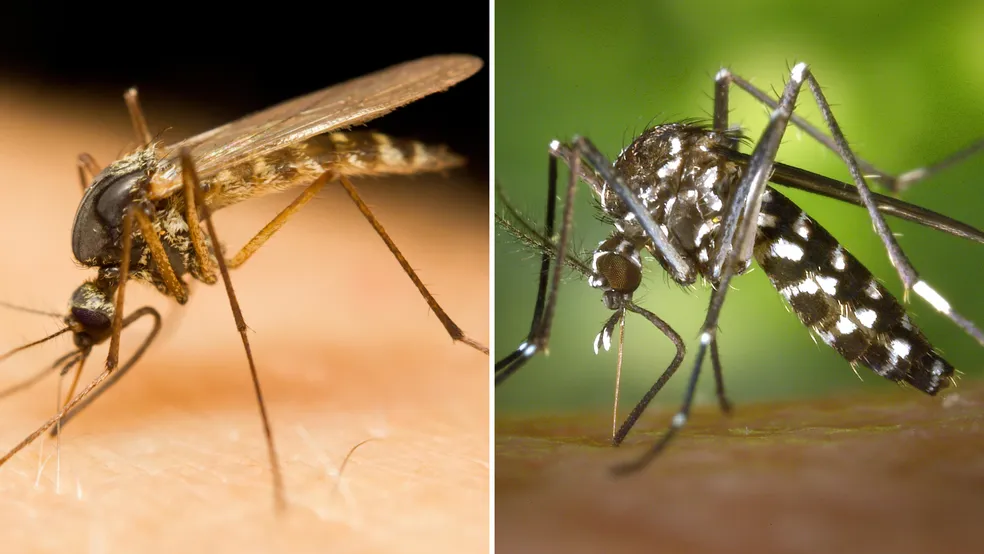
\includegraphics[width=0.5\linewidth]{Illustrations/aedes.png}
    \caption*{\textbf{Fonte: Globo Rural, 2023.}}
    \label{fig:enter-label}
\end{figure}
A enfermidade varia entre formas assintomáticas ou graves, levando a óbito. A maneira como a doença se manifesta em humanos pode variar de acordo com alguns fatores, como o vírus envolvido, infecção anterior pelo vírus da dengue e aspectos individuais, como doenças crônicas. O homem infectado pode apresentar sintomas de 2 a 7 dias, como febre, dor de cabeça, dor ao movimentar os olhos e dores musculares. Além destes, manchas vermelhas no corpo, vômitos e sangramentos no nariz ou nas gengivas podem ser um alerta para dengue hemorrágica. Os quatro sorotipos da dengue podem produzir formas assintomáticas e graves, mas os sorotipos 2 e 3 são considerados mais severos. \cite{7}. 
\begin{figure}[H]
    \centering
    \caption{Sintomas de dengue}
    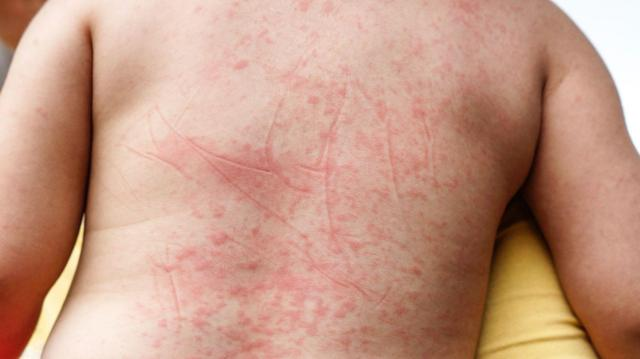
\includegraphics[width=0.5\linewidth]{Illustrations/sintomas.png}
    \caption*{\textbf{Fonte: BBC News Brasil, 2024.}}
    \label{fig:enter-label}
\end{figure}
Não há um tratamento específico ou remédios específicos para a dengue. O que pode ser feito é procurar suporte médico assim que os sintomas se manifestem para que ocorra um tratamento oportuno, a fim de minimizar o número de óbitos. \cite{8}. Uma alternativa é conter o criadouro do Aedes aegypti de maneira coletiva para reduzir a transmissão, eliminando água parada em pneus, garrafas vazias, potes, vasos de plantas ou qualquer outro objeto em que possa acumular água, além de realizar a limpeza da caixa d’água. \cite{9}.

Existem dificuldades relacionadas ao poder público que aceleram a transmissão da dengue. A primeira diz respeito ao fluxo rural-urbano ocorrido nos últimos anos, resultando em uma população de 124,1 milhões de pessoas nos centros urbanos até 2022. \cite{10}. Diante desse cenário, há uma falta de condições de habitação satisfatórias e saneamento básico por parte das cidades. Por essa razão, parte da população é submetida a um abastecimento de água e coleta de resíduos irregulares. Sem alternativas, a solução encontrada por essas pessoas é armazenar água para consumo, fator que favorece a proliferação do vetor. A produção de veículos também contribui para um maior número de pneus usados dispersos no meio ambiente. Outro empecilho referente ao poder público é a regularização do abastecimento de água e coleta de lixo em locais onde essas atividades não foram satisfatórias após o processo de fluxo rural-urbano, particularmente em comunidades carentes. O último ponto trata-se da pobre inspeção residencial, que abrange o cuidado ou eliminação de reservatórios potenciais do vetor. \cite{11}. 

Atualmente, os agentes de saúde já contribuem no combate às epidemias de dengue, alertando os moradores sobre os riscos e tratamentos dessa enfermidade, combatendo a eliminação de focos do Aedes aegypti e monitorando possíveis casos. Ademais, existem pesquisas dedicadas em tratar a dengue como uma endemia, realizando a contabilização de casos em distintas categorias por meio de gráficos ou mapas. No entanto, observa-se que os dados fornecidos por meio de aplicações já existentes representam apenas a última atualização, a qual pode ter ocorrido há três semanas, por exemplo \cite{20}. \cite{21}. \cite{22}. \cite{23}. Entretanto, há a carência de dados disponibilizados em tempo real para que os locais de foco das doenças sejam tratados de forma eficaz antes que a situação se agrave.

Dessa forma, a proposta do projeto é desenvolver um sistema de identificação de áreas de risco de dengue no Brasil. A aplicação consiste em desenvolver um sistema dedicado aos agentes de saúde, que poderão acessar um mapa para cadastrar o endereço residencial e o local de trabalho ou estudo de pessoas infectadas, além da localização de áreas com foco de dengue, como um pneu com água acumulada, por exemplo. Por outro lado, o gestor da equipe de agentes de saúde poderá ter acesso ao mapa de calor com os dados atualizados em tempo real, com o intuito de que a equipe de dedetização seja enviada para o tratamento do local.

A inteligência artificial (IA) é uma tecnologia que simula a capacidade humana de pensar, aprender e resolver problemas. Ela é usada em diversos campos para processar grandes quantidades de dados, tomar decisões rápidas e precisas, criar algoritmos e programas de computador. \cite{24}.

Com o intuito de promover a eficácia do sistema, o projeto em questão busca incluir a IA para cruzar as regiões afetadas de forma que estas sejam disponibilizadas de forma prioritária, ou seja, cada ponto representado no mapa receberá um nível de intensidade para determinar a ordem do processo de dedetização do ambiente e conter o avanço das doenças. Assim, a visualização dos dados e a eficácia no auxílio ao combate das epidemias de dengue podem ser aprimoradas. Este projeto é desenvolvido em colaboração com a prefeitura da cidade à qual se destina




\section*{OBJETIVO} \label{sect:obj}


O objetivo deste projeto é desenvolver um sistema para auxiliar os agentes de saúde a identificarem áreas infectadas pelo vetor da dengue. Por meio da IA, os gestores poderão analisar essas regiões no mapa disponível na aplicação, permitindo que uma equipe seja enviada ao local para a dedetização. Os principais objetivos deste projeto são: 

\begin{quote}
\begin{itemize}
    \raggedright
    \item[a)]Desenvolver um sistema de aplicativo móvel para facilitar a identificação de áreas com foco de dengue, apoiando ações de saúde pública e controle de doenças;
    \item[b)]Construir uma versão web para que os gestores responsáveis por visualizar o mapa possam observar as regiões mais afetadas, permitindo intervenções rápidas e eficazes para prevenir a propagação da doença;
    \item[c)]Fornecer dados em tempo real; 
    \item[d)]Contribuir na redução do número de óbitos por dengue no Brasil; 
\end{itemize}
\end{quote}
 

 \section*{ESTADO DA ARTE} \label{sect:estadoarte}

 Atualmente, a tecnologia tem desempenhado um papel fundamental no combate às doenças. A eficiência na análise de dados e a rápida troca de informações são essenciais para minimizar o número de vítimas durante crises de saúde. Nesta seção, apresentaremos alguns exemplos desses avanços e discutiremos como o Software EPIDEMIX se destaca em relação a outras tecnologias.

No estudo realizado T. et al. (2022), foram utilizadas informações médicas de pacientes com hanseníase fornecidas pelos Centros de Saúde Primária (PHCs) das cidades de Pamekasan e Pasuruan, na Indonésia. Em colaboração com uma equipe de pesquisadores e voluntários, Taal realizou visitas domiciliares aos pacientes para coletar suas coordenadas geográficas (latitude e longitude) utilizando a aplicação MapIt, que usa o Geographic Positioning Systems (GPS) para a coleta dos dados. Essas coordenadas foram processadas pelo sistema de código-aberto Quantum Geographic Information System (QGIS), e os agrupamentos de casos de hanseníase foram calculados utilizando o programa ClusterSeer. Em seguida, a ferramenta de mapa de calor do QGIS foi empregada para gerar uma representação visual da distribuição dos casos com base em diferentes níveis de densidade.

O estudo identificou um grande agrupamento de casos em Pamekasan e Pasuruan, com quase 100\% dos casos localizados dentro das áreas destacadas no mapa de calor. Estima-se que entre 21\% e 90\% dos casos futuros estarão dentro das áreas identificadas. Essas informações podem ser usadas para melhorar a eficácia das estratégias de combate e prevenção dessas doenças.

Em Miguel, Hornink e Bressan (2020), Miguel desenvolve um aplicativo móvel destinado a identificar e visualizar áreas de foco para Dengue, Zika e Chikungunya em um mapa, seja através de pontos individuais ou mapas de calor. Os usuários podem inserir um registro de foco a qualquer momento, simplesmente pressionando no mapa na tela inicial do aplicativo. As informações sobre a localização dos focos são armazenadas em um banco de dados, processadas e, em seguida, exibidas na interface do mapa do aplicativo, que também oferece a opção de filtrar por tipo de registro ou por período. No entanto, os dados utilizados para demonstrar o aplicativo eram fictícios, deixando uma lacuna na validação prática do software em situações reais. Embora a ferramenta tenha demonstrado eficácia teórica, não foram consideradas a possibilidade de registros falsos pelos usuários ou registros repetidos, já que mais de uma pessoa poderia registrar o mesmo local, resultando na criação de uma grande área de risco falsa. Ambas as possibilidades podem impactar negativamente a precisão das informações apresentadas.





 \section*{METODOLOGIA} \label{sect:metodologia}

 O estudo propõe um sistema dedicado à identificação de áreas de risco de dengue no Brasil. Seu propósito é fornecer suporte aos agentes de saúde para que a dedetização dos locais aconteça de forma eficiente. A fim de que o sistema seja satisfatório, algumas técnicas que serão utilizadas são cruciais, como suavizar os pontos afetados em um HeatMap para facilitar a visualização, além de fornecer rotas eficazes aos agentes de dedetização para que mais regiões sejam tratadas em menos tempo, auxiliando no combate à proliferação dessa doença. A metodologia deste estudo envolve o uso de IA para que as técnicas citadas possam ser aplicadas ao projeto, assim como ferramentas de design e desenvolvimento de software. 

Para a criação da interface do usuário do software EPIDEMIX, empregamos o Figma. Este software de design gráfico permite a criação de protótipos interativos de baixa e alta fidelidade, com layouts e estilos, facilitando a elaboração do design de forma clara aos usuários e permitindo modificações conforme necessário.

Além disso, utilizamos a plataforma SEBRAE Canvas para planejar o modelo de negócios do software. Esta plataforma fornece um quadro dividido em seções como parcerias, proposta de valor, estrutura de custos e fontes de receita, auxiliando no planejamento de cada aspecto do modelo de negócios e na definição dos elementos-chave do projeto. É importante citar que o Canvas do projeto foi desenvolvido antes mesmo do aplicativo, pois a partir dele uma visão lógica e completa do sistema pode ser concebida.

Com o auxílio do brModelo, criamos o modelo conceitual e lógico do banco de dados necessário para o funcionamento do EPIDEMIX. O brModelo é um software que facilita a criação dos modelos de um banco de dados usando diagramas de entidade-relacionamento (DER). Com os modelos finalizados, é possível desenvolver a interface do aplicativo, garantindo uma compreensão detalhada do funcionamento de cada entidade do sistema e de suas interações.

Por meio do LucidChart foi criado o diagramas de caso de uso UML do sistema, devido à sua interface intuitiva e ampla gama de recursos específicos para UML, que facilitam a representação visual precisa dos requisitos funcionais do projeto. Sua capacidade de colaboração em tempo real permite uma colaboração eficiente entre os membros da equipe.

A plataforma Draw.io foi empregada para a construção do diagrama de redes do sistema proposto. O Draw.io é uma ferramenta online de diagramação que oferece uma interface intuitiva e uma ampla gama de recursos para criação de diagramas profissionais em diversas áreas, incluindo redes de sistemas. O uso da plataforma proporcionou uma abordagem eficaz para a criação do diagrama de redes do sistema estudado, permitindo uma representação visual clara e precisa de sua infraestrutura de rede.

Para criar o sistema desktop inicialmente utilizamos o Apex da Oracle, uma plataforma de desenvolvimento de aplicativos baseada em banco de dados. O Apex permite criar rapidamente aplicativos web escaláveis, aproveitando a potência do Oracle Database. Com sua interface de desenvolvimento intuitiva e ferramentas integradas, o Apex agiliza o processo de desenvolvimento e oferece flexibilidade para atender às necessidades específicas do sistema. Porém, demos continuidade na criação do sistema desktop utilizando a linguagem de programação Java Script através do programa Visual Studio Code e a plataforma Node.js.

O Visual Studio Code foi escolhido como ambiente de desenvolvimento pela sua interface intuitiva e pela ampla gama de extensões que otimizam a produtividade, enquanto o Node.js foi utilizado para construir o backend do sistema. A escolha do Node.js possibilitou a criação de uma estrutura de backend robusta, que oferece alta performance e escalabilidade, fundamentais para suportar o crescimento do sistema.

A combinação dessas ferramentas trouxe flexibilidade ao desenvolvimento, permitindo integrações com outras tecnologias e ampliando a capacidade de personalização do sistema para atender melhor às necessidades dos usuários. Dessa forma, a equipe conseguiu manter um fluxo de trabalho ágil e otimizado para desenvolver novas funcionalidades e aperfeiçoar a experiência final do sistema.

 \section*{RESULTADOS PRELIMINARES}\label{sect:resultados}

 Embora o sistema não esteja operacional e aplicado de forma prática em um contexto real, o estudo apresentado até aqui mostra-se capaz de fornecer informações precisas sobre os locais afetados pela dengue aos agentes de saúde, de forma a contribuir com os objetivos propostos. Futuramente pretende-se realizar pesquisas de campo com os agentes de saúde para testar a usabilidade do aplicativo. Mesmo sem os resultados das pesquisas de campo, acredita-se que o projeto possa ajudar os agentes e gestores de saúde para garantir a dedetização eficaz dos locais de risco.\newline

\textbf{Sistema feito em Java}\newline
A (Figura 3) Esta tela representa a interface inicial do aplicativo, antes de realizar o login.

\begin{figure}[H]
    \centering
    \caption{Tela 1}
    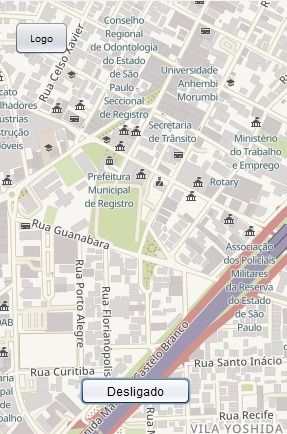
\includegraphics[width=0.5\linewidth]{Illustrations/Visi_Seco.jpg}
    \caption*{\textbf{Fonte: do próprio autor, 2024.}}
\end{figure}

\vspace{12pt}

A (Figura 4) Esta é a tela inicial do administrador, onde ele pode selecionar a doença que deseja visualizar no HeatMap, escolher a rota para enviar as equipes de dedetização e registrar uma localização de dengue.

\begin{figure}[H]
    \centering
    \caption{Tela 2}
    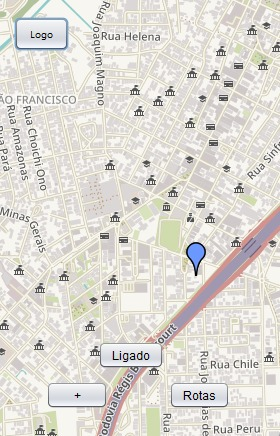
\includegraphics[width=0.5\linewidth]{Illustrations/Adm.jpg}
    \caption*{\textbf{Fonte: do próprio autor, 2024.}}
\end{figure}

\vspace{12pt}

 A (Figura 5) mostra a tela inicial do agente de saúde, o qual pode registar uma localização de foco de dengue e visualizar o HeatMap da doença.
 
\begin{figure}[H]
    \centering
    \caption{Tela 3}
    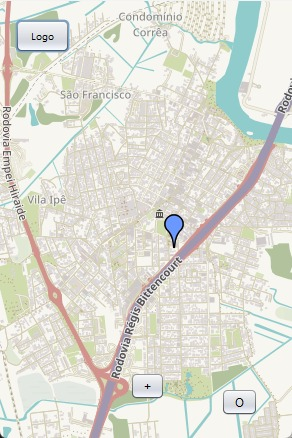
\includegraphics[width=0.5\linewidth]{Illustrations/Agente.jpg}
    \caption*{\textbf{Fonte: do próprio autor, 2024.}}
\end{figure}

\vspace{12pt}

A (Figura 6) indica a tela inicial do agente de dedetização, o qual terá acesso às possíveis rotas para o tratamento dos focos.

\begin{figure}[H]
    \centering
    \caption{Tela 4}
    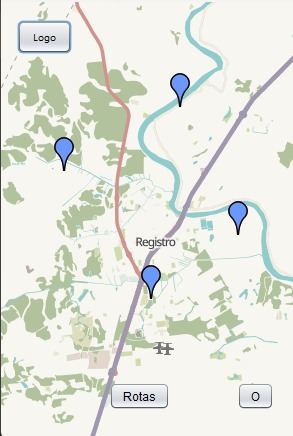
\includegraphics[width=0.5\linewidth]{Illustrations/Dedetizador.jpg}
    \caption*{\textbf{Fonte: do próprio autor, 2024.}}
\end{figure}

\vspace{12pt}

A (Figura 7) ilustra a tela inicial do visitante, o qual terá acesso apenas aos mapas de calor de dengue.

\begin{figure}[H]
    \centering
    \caption{Tela 5}
    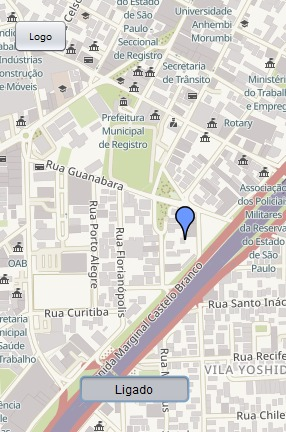
\includegraphics[width=0.5\linewidth]{Illustrations/Visitante.jpg}
    \caption*{\textbf{Fonte: do próprio autor, 2024.}}
\end{figure}

\vspace{12pt}

A (Figura 8) representa o mapa de calor da dengue. O mapa poderá ser visualizado pelo administrador, pelo agente de saúde e pelo visitante. 


\begin{figure}[H]
    \centering
    \caption{Tela 7}
    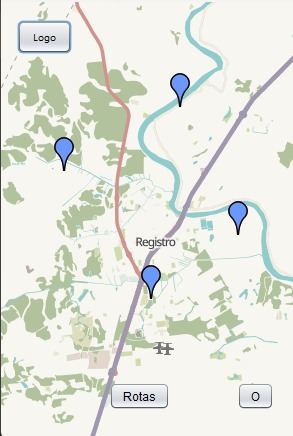
\includegraphics[width=0.5\linewidth]{Illustrations/mapa_calor.jpg}
    \caption*{\textbf{Fonte: do próprio autor, 2024.}}
\end{figure}

A (Figura 9) ilustra a tela de registro de localização de foco de dengue, atividade que poderá ser realizada pelo administrador ou agente de saúde.

\begin{figure}[H]
    \centering
    \caption{Tela 9}
    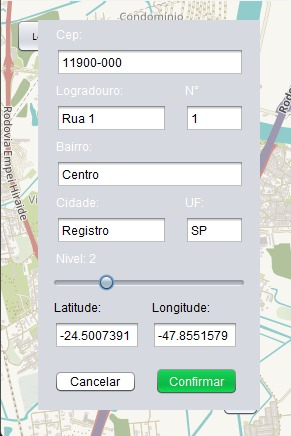
\includegraphics[width=0.5\linewidth]{Illustrations/Agt_cad.jpg}
    \caption*{\textbf{Fonte: do próprio autor, 2024.}}
\end{figure}


\vspace{12pt}

\textbf{Sistema em Node}\newline

O sistema foi inicialmente desenvolvido em Apex para facilitar a construção e visualização da aplicação web executável. A aplicação em Node.js visa proporcionar ao administrador uma visão geral da plataforma. Ela oferece ao gestor acesso total aos dados do sistema, permitindo a visualização dos agentes cadastrados, suas respectivas permissões e os celulares atribuídos a cada um. Além disso, o sistema registra os endereços onde foram identificados focos de dengue, acompanhados dos respectivos mapas de calor.

Essa abordagem visa fornecer ao administrador uma ferramenta eficiente para monitorar e gerenciar todos os aspectos relevantes da aplicação.

\vspace{12pt}

A (Figura 10) representam a aba de inserção do registro de um local com foco de dengue.

\begin{figure}[H]
    \centering
    \caption{Registro dengue}
    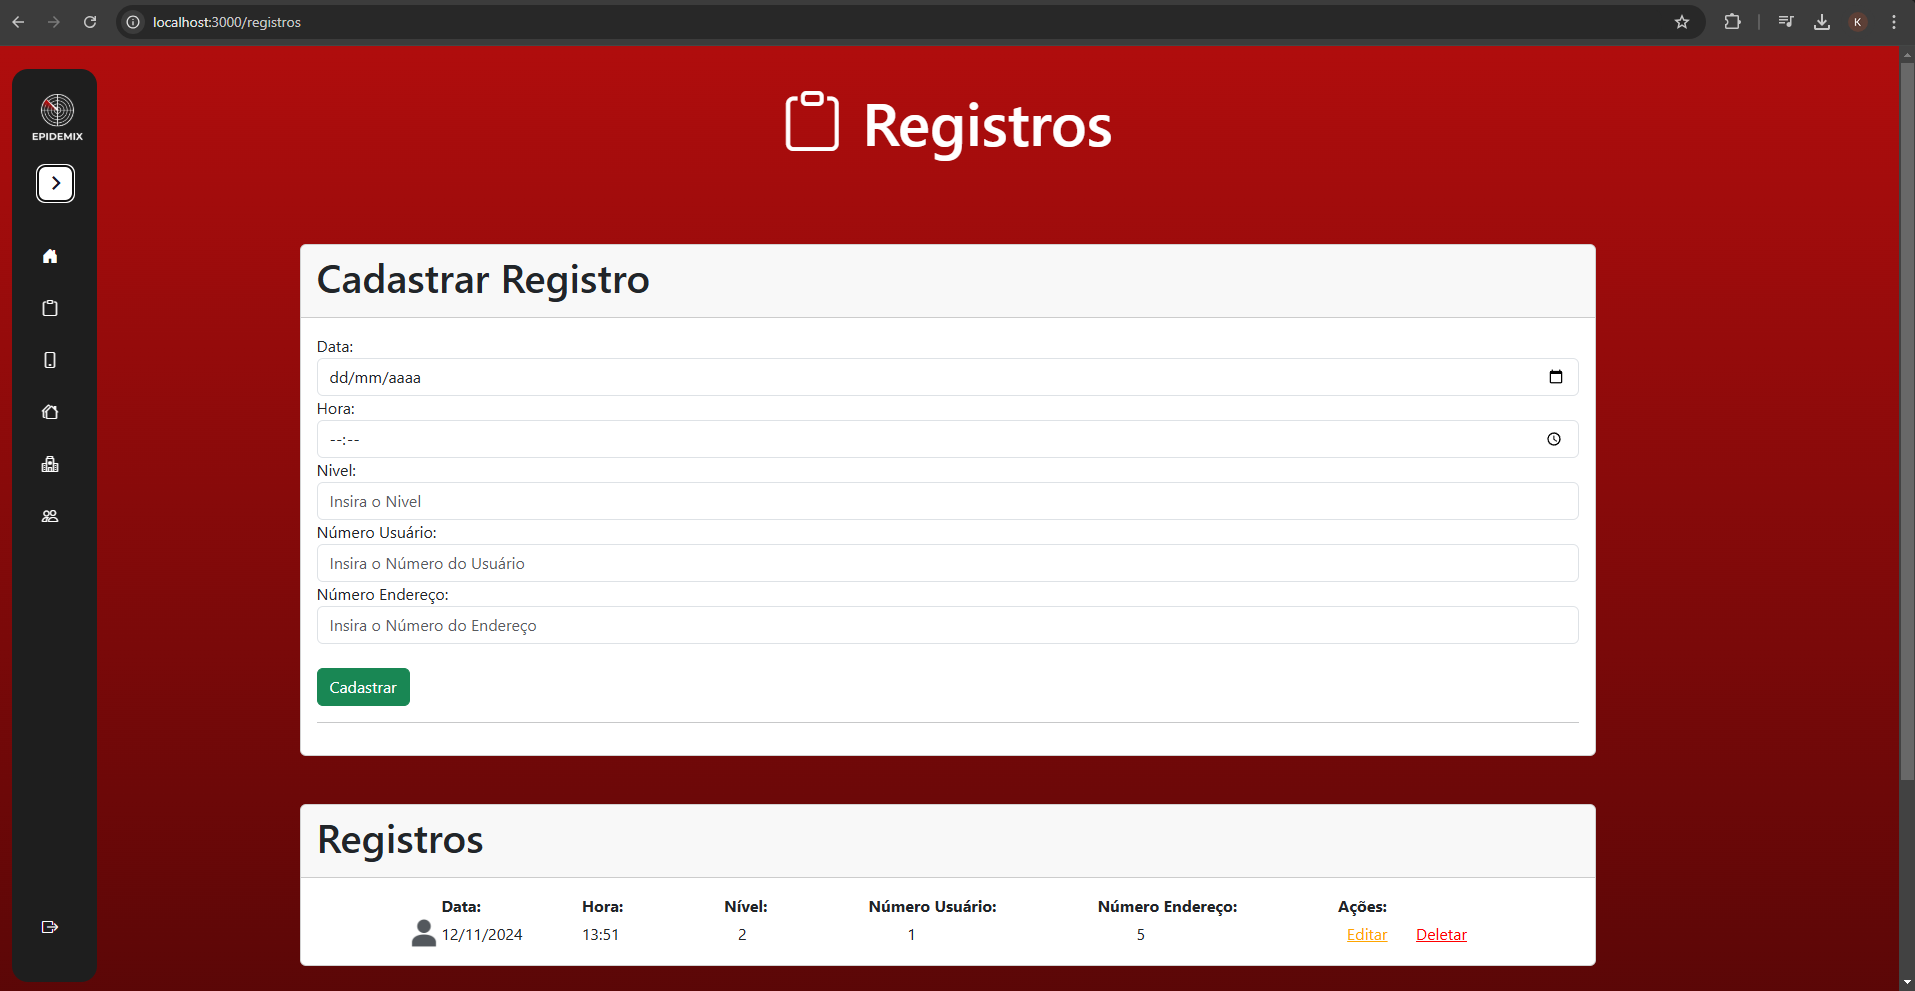
\includegraphics[width=1.0\linewidth]{Illustrations/Registro_Epidemix.png}
    \caption*{\textbf{Fonte: do próprio autor, 2024.}}
\end{figure}

\vspace{12pt}

A (Figura 11) mostra o mapa de calor de dengue com os pontos afetados por foco das doenças. 

\begin{figure}[H]
    \centering
    \caption{Mapa de calor dengue}
    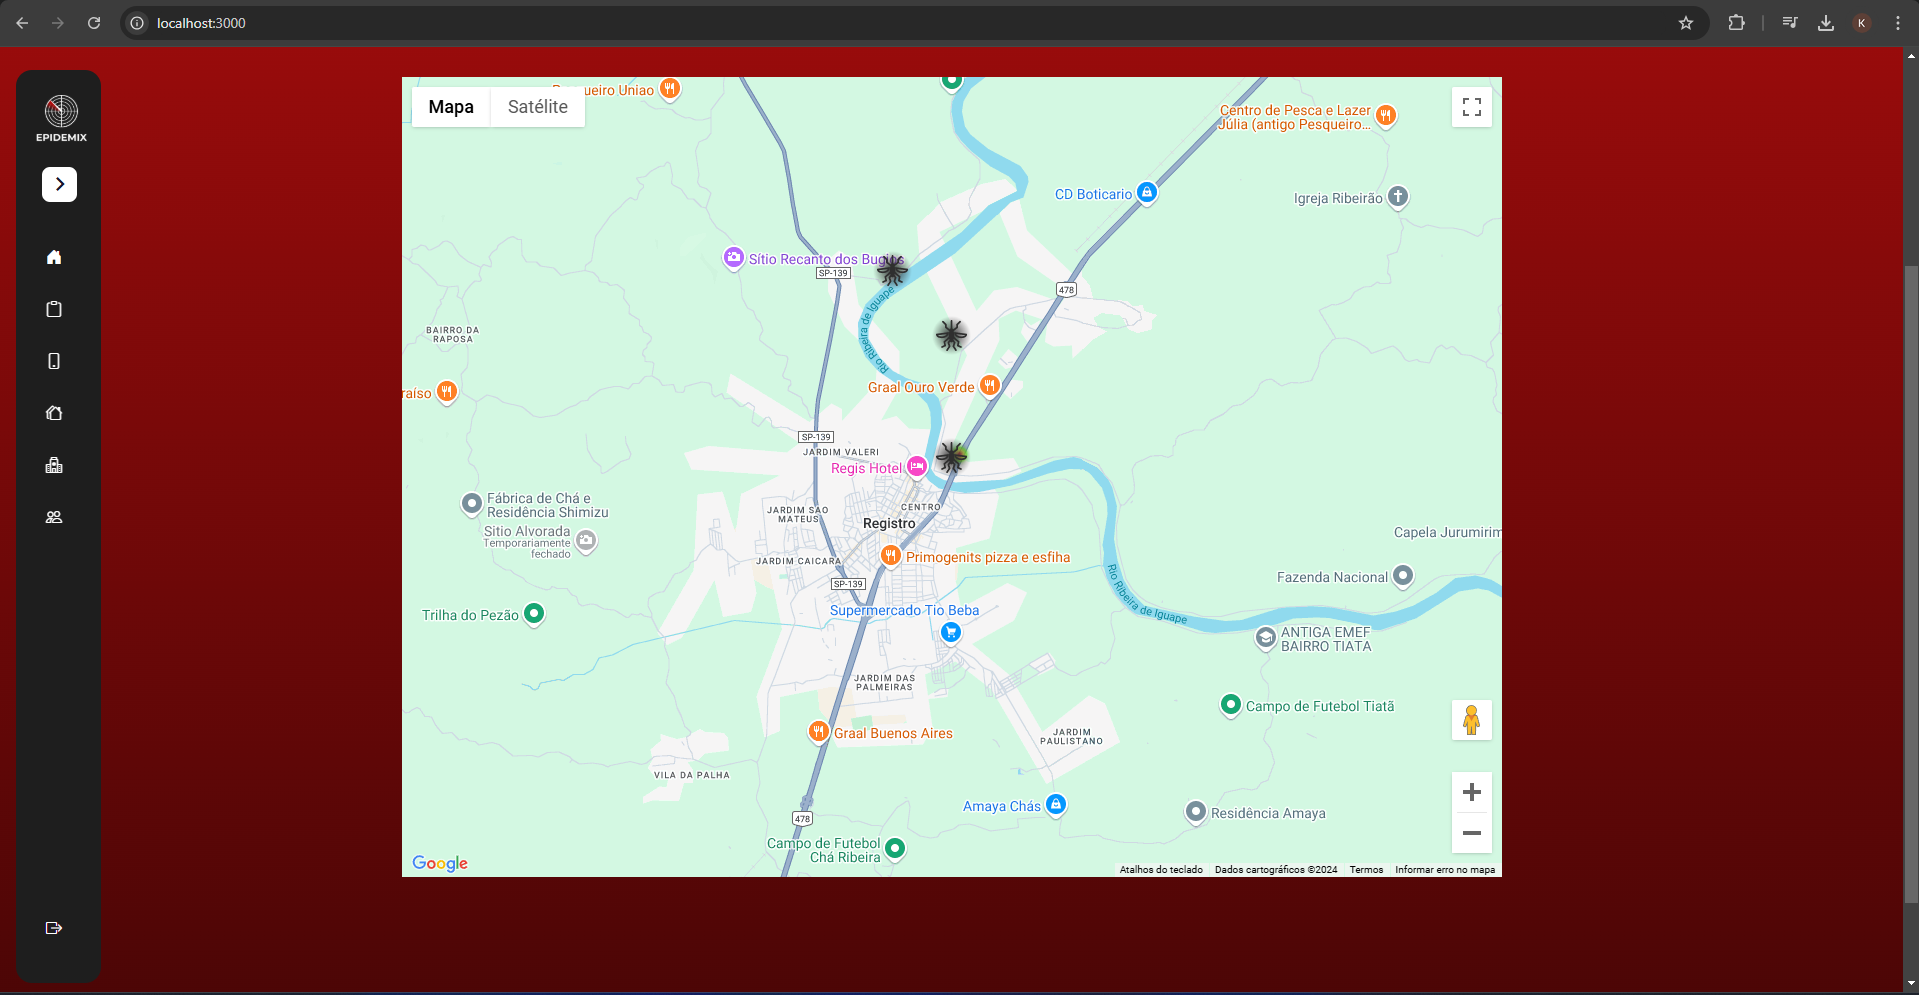
\includegraphics[width=1.0\linewidth]{Illustrations/Mapa de Calor.png}
    \caption*{\textbf{Fonte: do próprio autor, 2024.}}
\end{figure}

\vspace{12pt}


Na (Figura 12 e 13) é possível obervar os usuários e os celulares cadastrados. No caso, os usuários são os agentes e os celulares são os dispositivos utilizados para registrar uma localização.

\begin{figure}[H]
    \centering
    \caption{Usuários}
    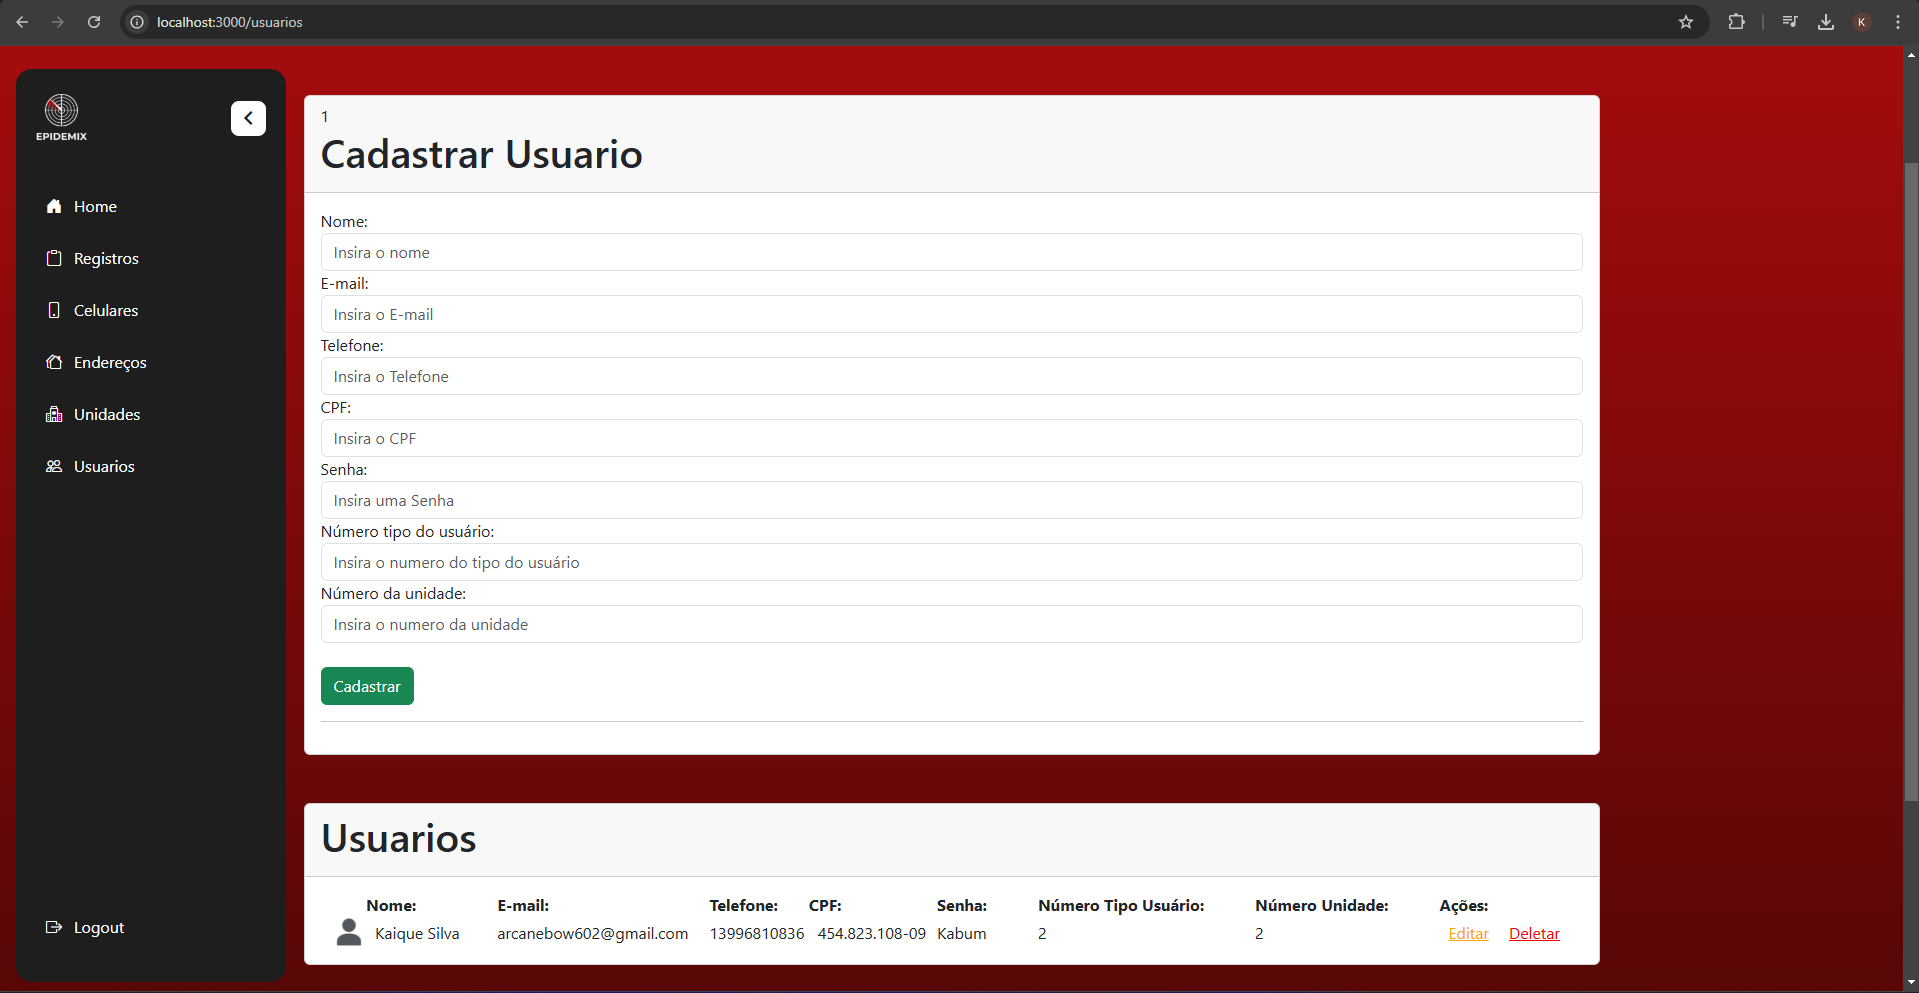
\includegraphics[width=1.0\linewidth]{Illustrations/Usuario.png}
    \caption*{\textbf{Fonte: do próprio autor, 2024.}}
\end{figure}

\vspace{12pt}

\begin{figure}[H]
    \centering
    \caption{Celulares}
    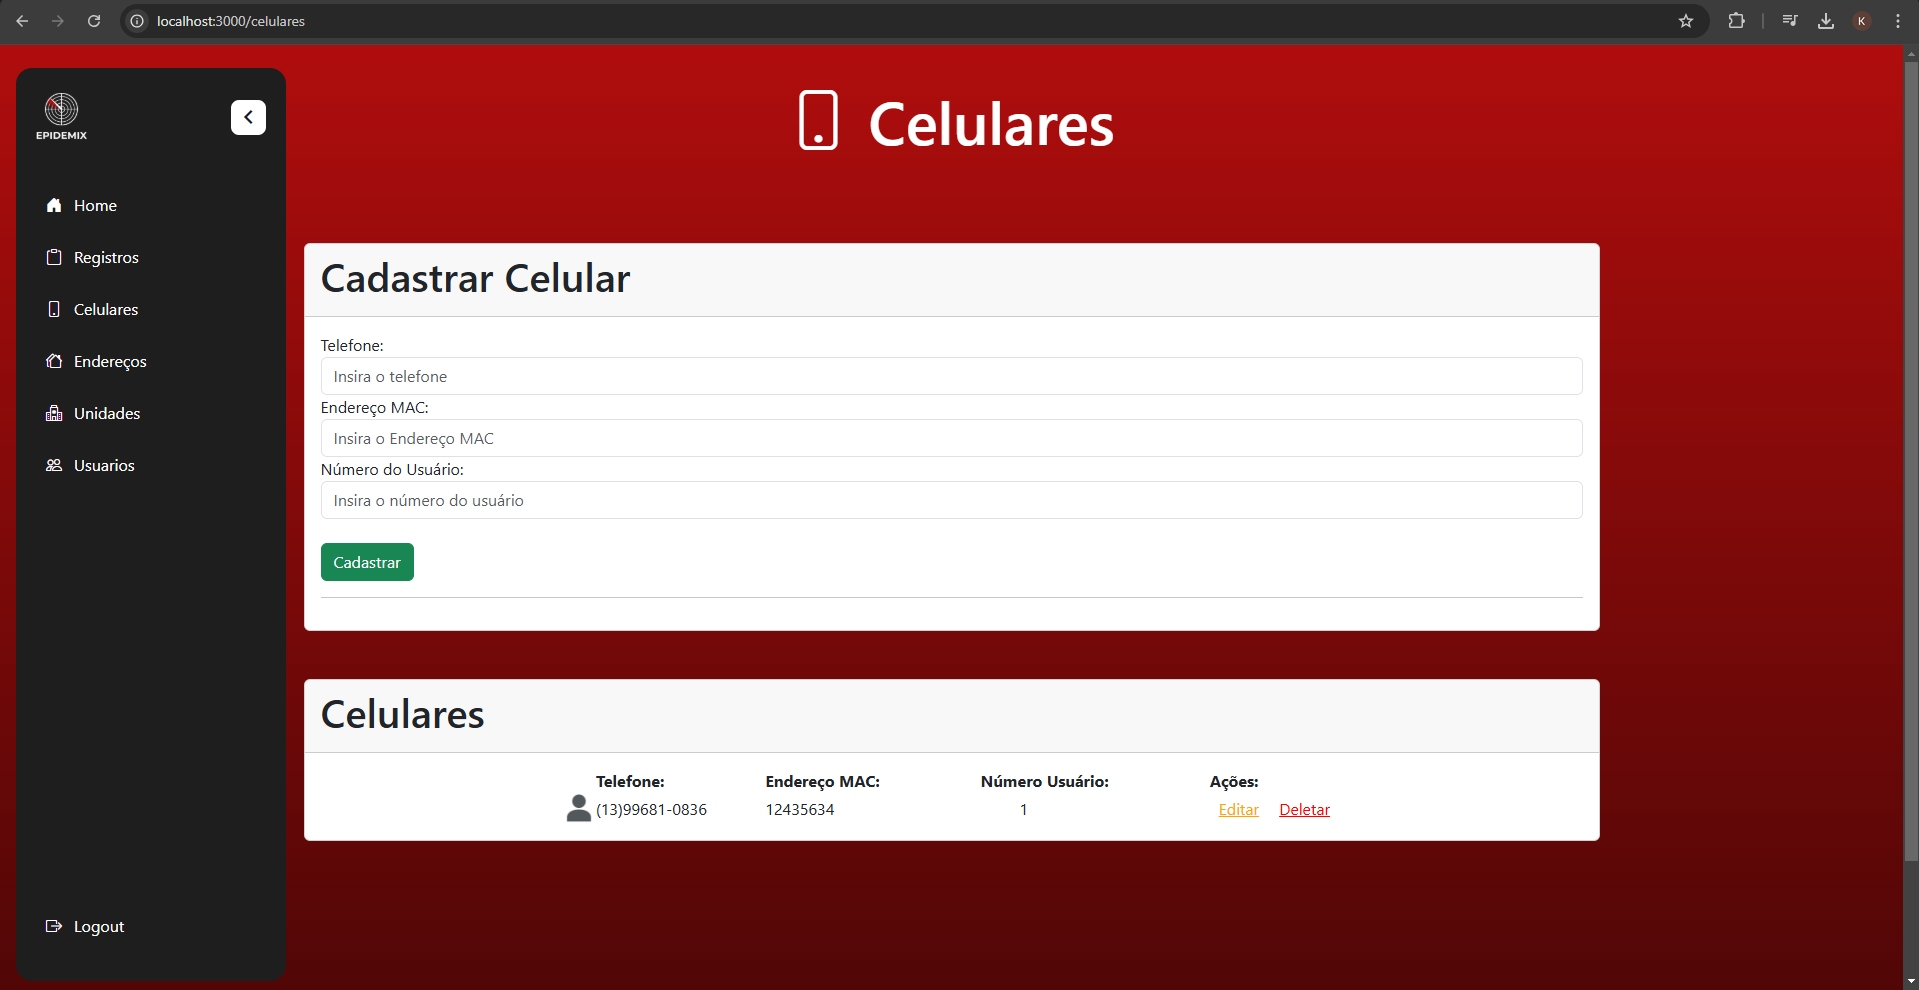
\includegraphics[width=1.0\linewidth]{Illustrations/celulares.png}
    \caption*{\textbf{Fonte: do próprio autor, 2024.}}
\end{figure}

\vspace{12pt}

A (Figura 14) mostra a aba Endereços, onde é possível observar as informações de uma localização afetada, como o endereço do local, o nível do risco e o agente responsável pelo registro. 

\begin{figure}[H]
    \centering
    \caption{Endereços}
    \includegraphics[width=1.0\linewidth]{Illustrations/Endereços.png}
    \caption*{\textbf{Fonte: do próprio autor, 2024.}}
\end{figure}

\vspace{12pt}

A (Figura 15) representa as unidades em que a equipe responde.

\begin{figure}[H]
    \centering
    \caption{Unidades}
    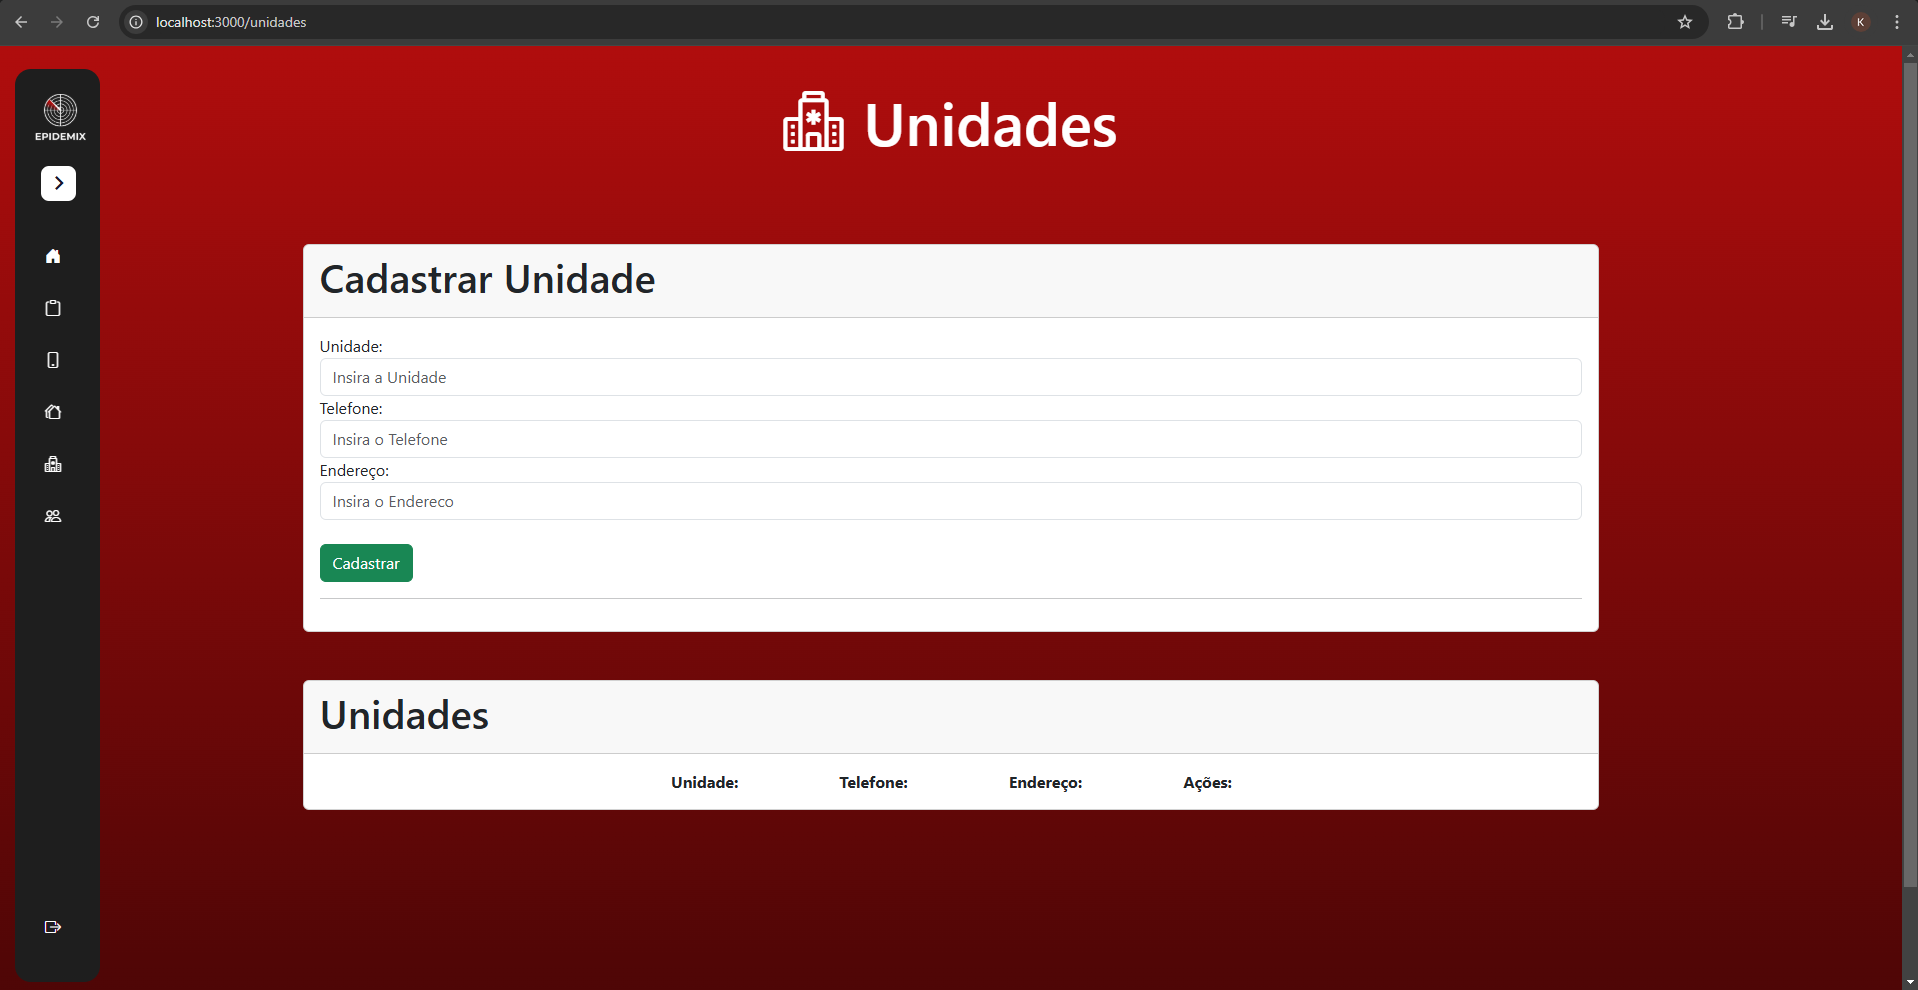
\includegraphics[width=1.0\linewidth]{Illustrations/Unidades.png}
    \caption*{\textbf{Fonte: do próprio autor, 2024.}}
\end{figure}

\vspace{12pt}


\textbf{Diagrama de caso de uso}\newline

A UML (Unified Modeling Language) do sistema serve para visualizar, especificar e documentar a estrutura e o comportamento externo do sistema de software. O diagrama fornece uma linguagem padronizada para comunicar as diferentes partes e aspectos que o sistema irá oferecer aos usuários, auxiliando no projeto, desenvolvimento e manutenção do software. 

Durante o desenvolvimento da UML, seis atores foram identificados. O super administrador, que faz referência ao dono do software, depende que o administrador envie dados pessoais e dados do departamento ao qual ele está cadastrado, para que o dono possa gerenciar os dados inseridos. Além disso, outras funcionalidades podem ser atribuídas a ele, como o gerenciamento do cadastro de um agente de saúde, o registro da localização afetada, a edição dos dados inseridos, e a criação e observação de relatórios. Outro ator reconhecido é o administrador/coordenador da equipe de saúde, responsável por administrar cadastros de agentes de saúde e por gerar e visualizar os relatórios. O registro da localização afetada e a edição de tais dados são outras funcionalidades que podem ser atribuídas a ele. O próximo ator é o agente de saúde, que envia dados pessoais para que o coordenador e o super administrador possam gerenciá-los. Sua principal função é registrar uma área com foco de dengue, mas também poderá visualizar os relatórios gerados pelos dados inseridos no sistema. O usuário civil foi identificado, este poderá apenas visualizar os mapas gerados com a intenção de reconhecer áreas afetadas e preservar sua saúde.

\begin{figure}[H]
    \centering
    \caption{Diagrama de caso de uso}
    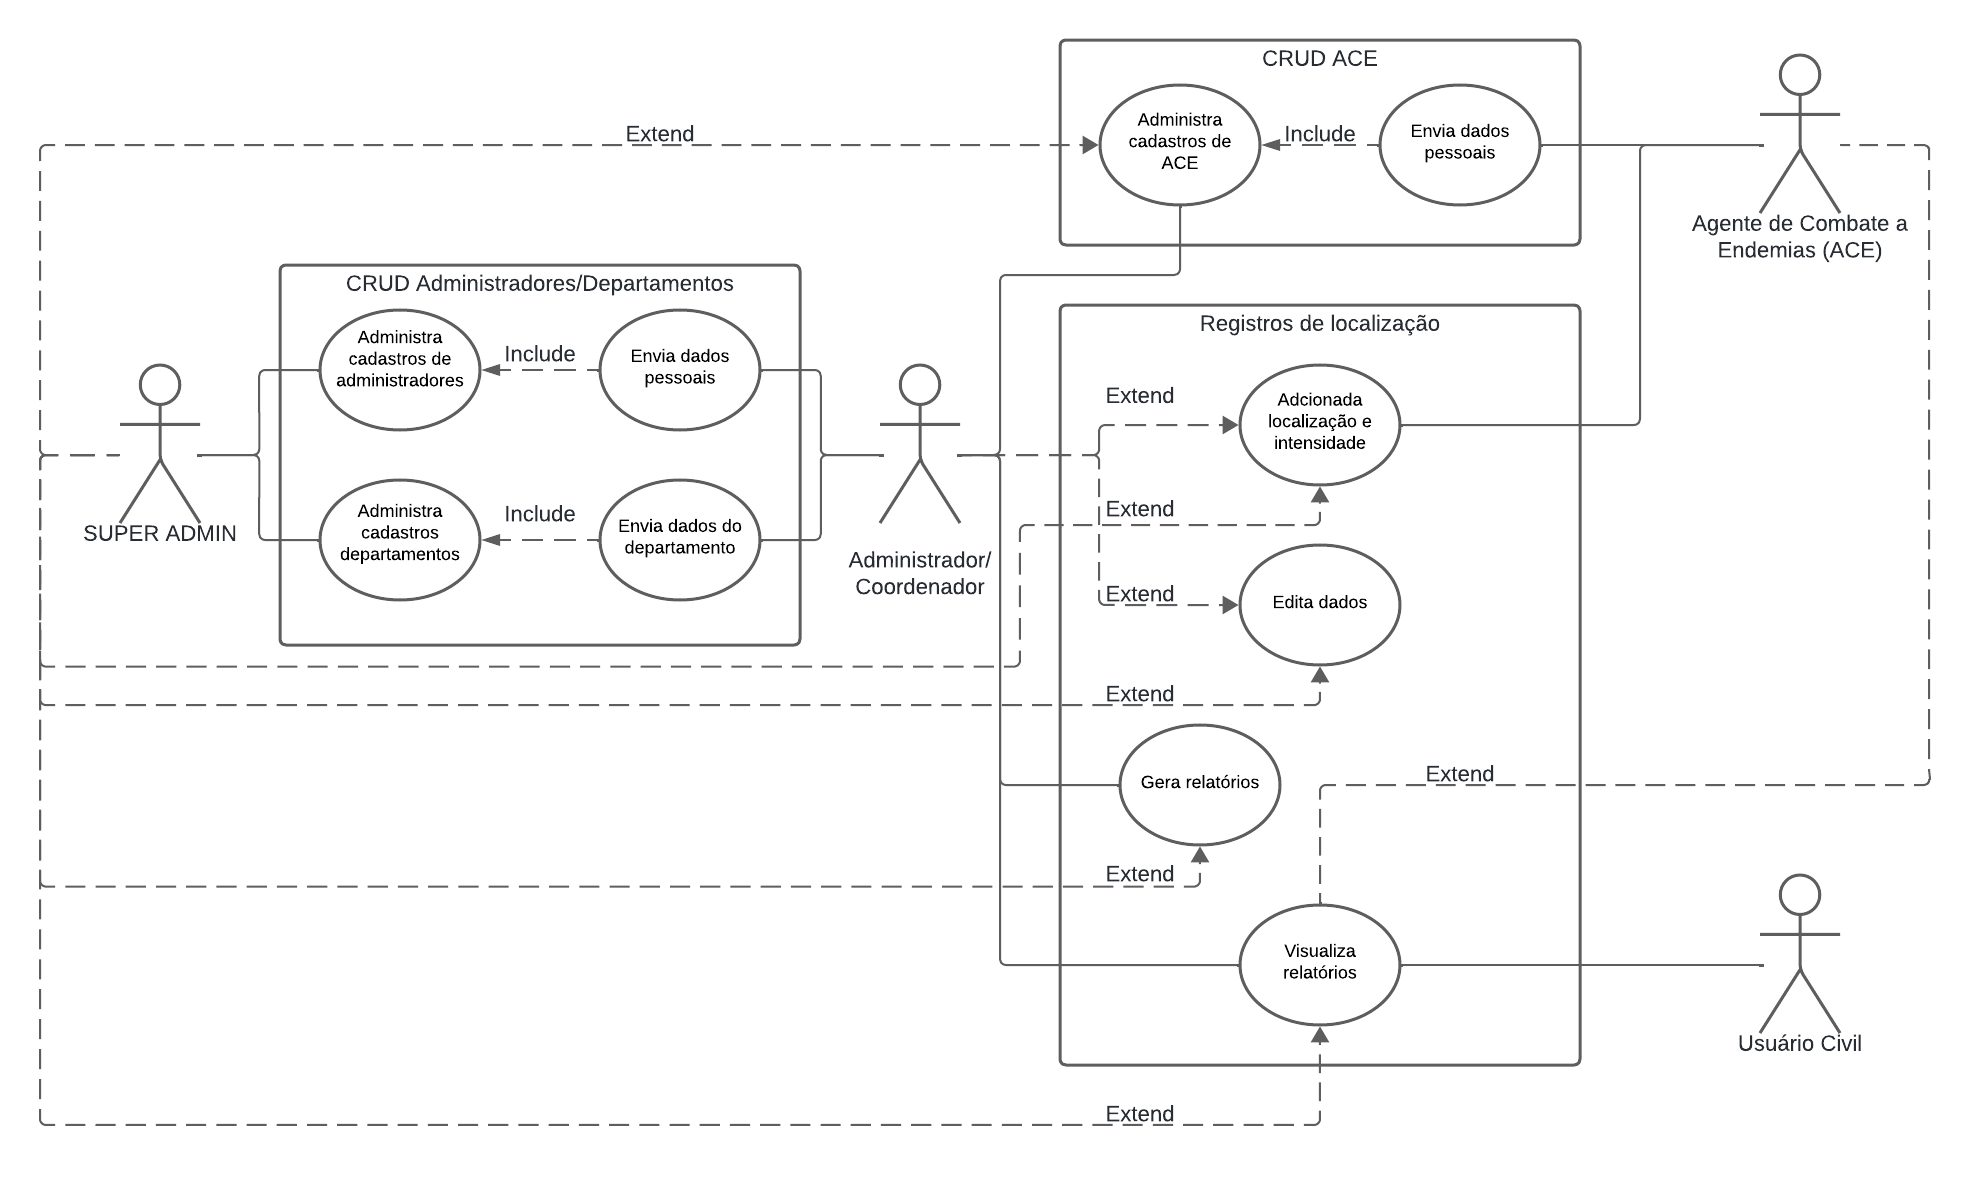
\includegraphics[width=1.0\linewidth]{Illustrations/uml1.png}
    \caption*{\textbf{Fonte: do próprio autor, 2024.}}
\end{figure}

\vspace{12pt}

Na continuação da UML, o gestor da equipe de saúde visualiza e encaminha as rotas geradas pela inteligência artificial para o agente dedetizador para que o tratamento do local possa ser realizado. Ainda cabe ao coordenador administrar os cadastros do agente dedetizador. Este, por sua vez, envia seus dados pessoais ao administrador, visualiza e finaliza as rotas de tratamento. A finalização da rota também pode ser realizada pelo coordenador. 

\begin{figure}[H]
    \centering
    \caption{Diagrama de caso de uso}
    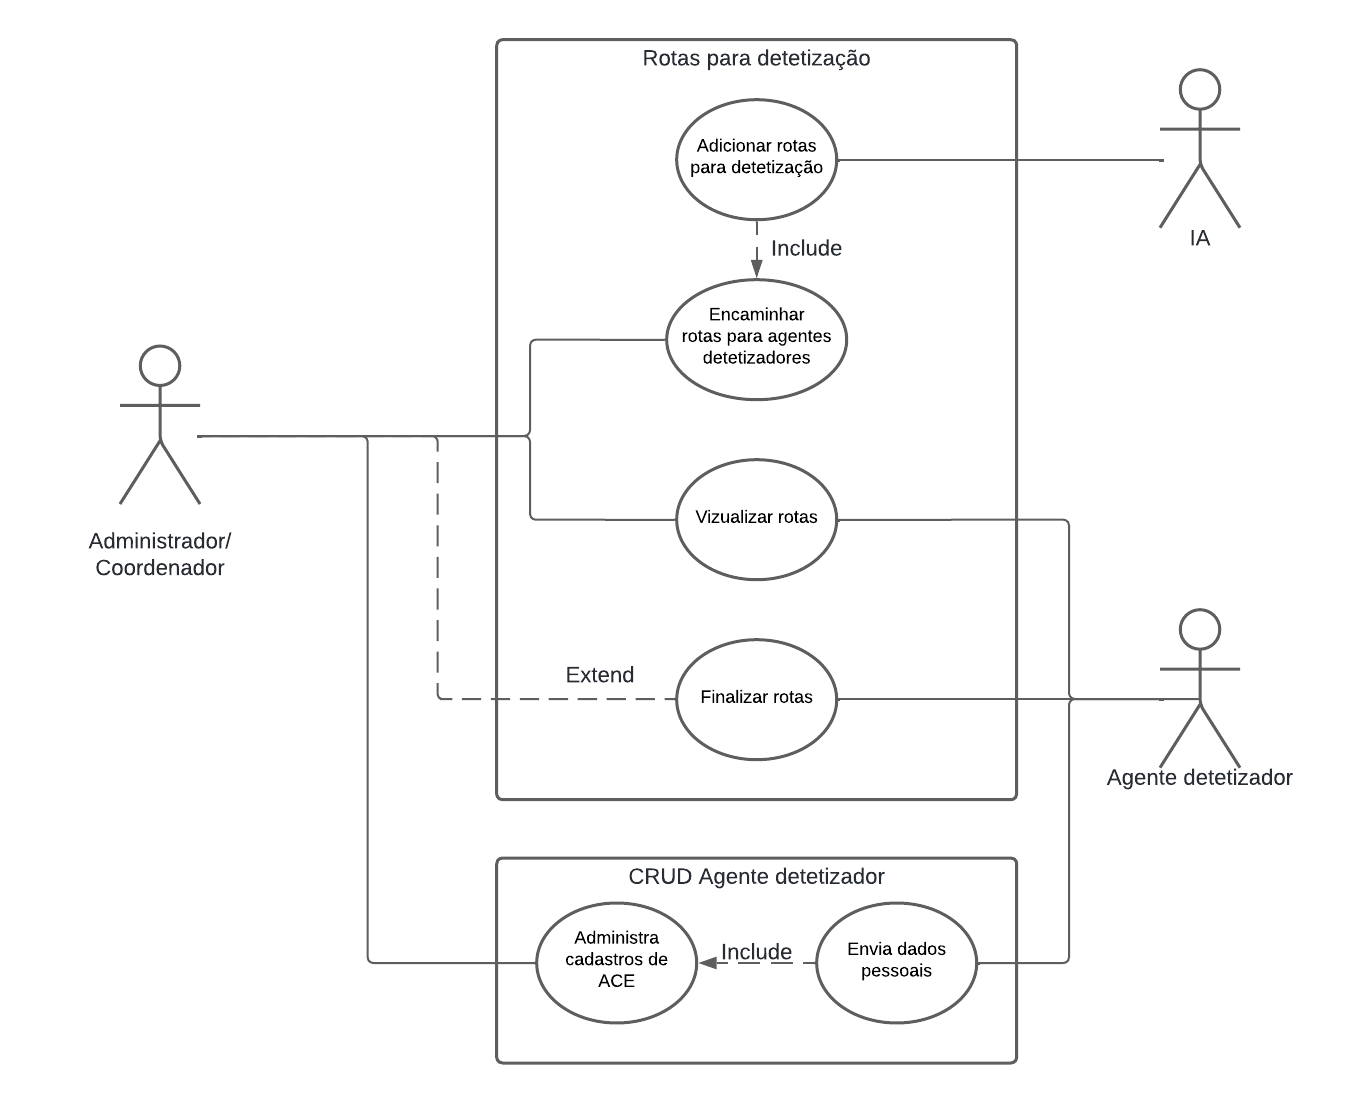
\includegraphics[width=1.0\linewidth]{Illustrations/uml2.png}
    \caption*{\textbf{Fonte: do próprio autor, 2024.}}
\end{figure}

\vspace{12pt}

É importante observar que foram criados dois diagramas separados, pois a plataforma em que foram desenvolvidos possui limite de elementos a serem utilizados. 

\vspace{12pt}

\textbf{Diagrama de redes}\newline

O diagrama de redes do sistema serve como uma representação visual da infraestrutura de rede, destacando dispositivos, conexões e a topologia geral. Sendo assim, facilita a compreensão da arquitetura da rede, ajudando na identificação de componentes individuais e suas interconexões. Em suma, o diagrama de redes é essencial para gerenciamento eficaz da infraestrutura de rede da aplicação. 

O diagrama de redes foi estruturado da seguinte forma: o agente de saúde acessa o aplicativo através do celular por meio da rede, e, consequentemente, qualquer alteração feita por ele será armazenada na nuvem. Por outro lado, o administrador terá acesso total à infraestrutura de rede, ou seja, será capaz de visualizar as alterações feitas pelo agente e salvas na nuvem, refletidas no aplicativo EPIDEMIX armazenado no servidor.

\begin{figure}[H]
    \centering
    \caption{Diagrama de redes}
    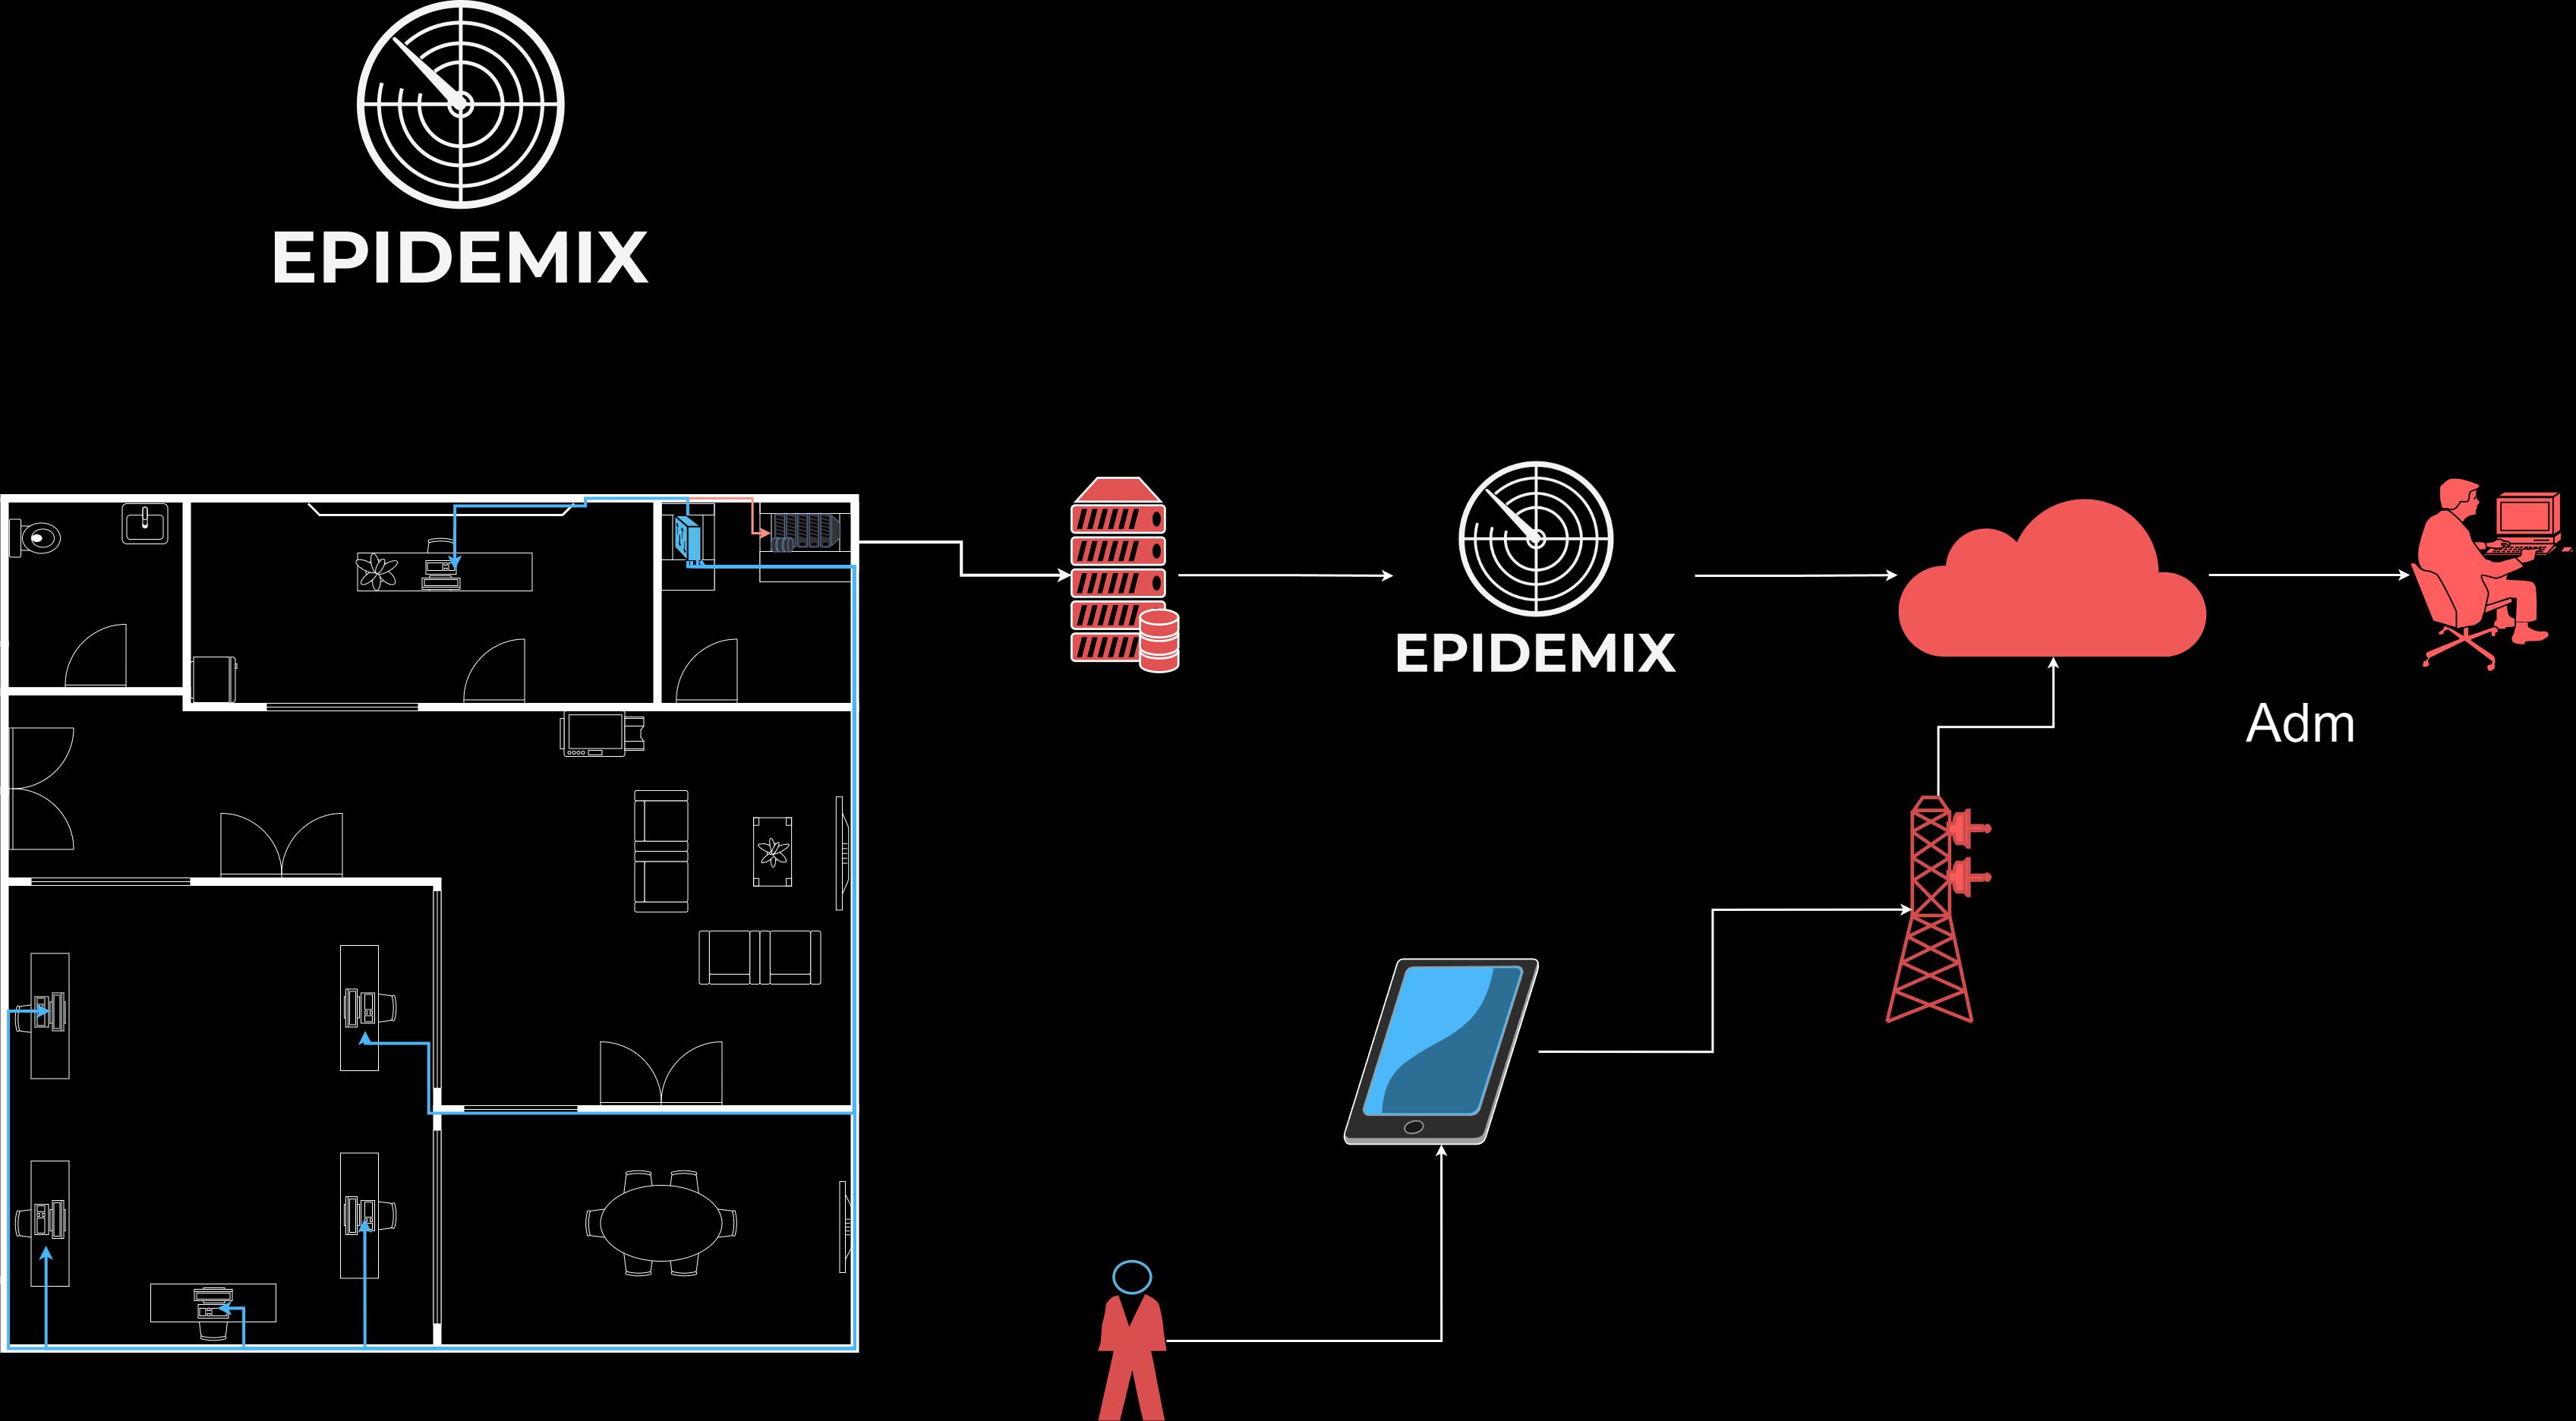
\includegraphics[width=1.0\linewidth]{Illustrations/redes.png}
    \caption*{\textbf{Fonte: do próprio autor, 2024.}}
\end{figure}

\vspace{12pt}

\textbf{Modelagem de banco de dados}\newline

O modelo de banco de dados conceitual delineia os requisitos de dados de forma abstrata, facilitando a compreensão dos relacionamentos entre entidades no sistema. Já o modelo lógico traduz esses conceitos em estruturas de dados concretas, permitindo sua implementação técnica. Juntos, esses modelos fornecem uma base sólida para o design e desenvolvimento do banco de dados da aplicação, garantindo consistência e eficiência. 

Ao acessar o aplicativo, o usuário irá realizar o login na seção em que ele se enquadra, fazendo referência à entidade "Tipos-usuário". O tipo de usuário varia entre administrador da equipe, agente de saúde, agente de dedetização e visitante, os quais possuem suas respectivas permissões. O Usuário já estará cadastrado na entidade "Users" com as seguintes informações: nome completo, e-mail, telefone, CPF e senha. Cada profissional terá um celular vinculado a ele de acordo com o endereço MAC do aparelho, e também estará relacionado à unidade a qual ele responde, o hospital será identificado pelo nome e telefone de contato. Após o usuário realizar o login com seu e-mail e senha, poderá fazer o registro da localização de dengue. No registro da doença é necessário inserir o endereço, a data, a hora e o nível do foco identificado.

\begin{figure}[H]
    \centering
    \caption{Banco de dados modelo conceitual}
    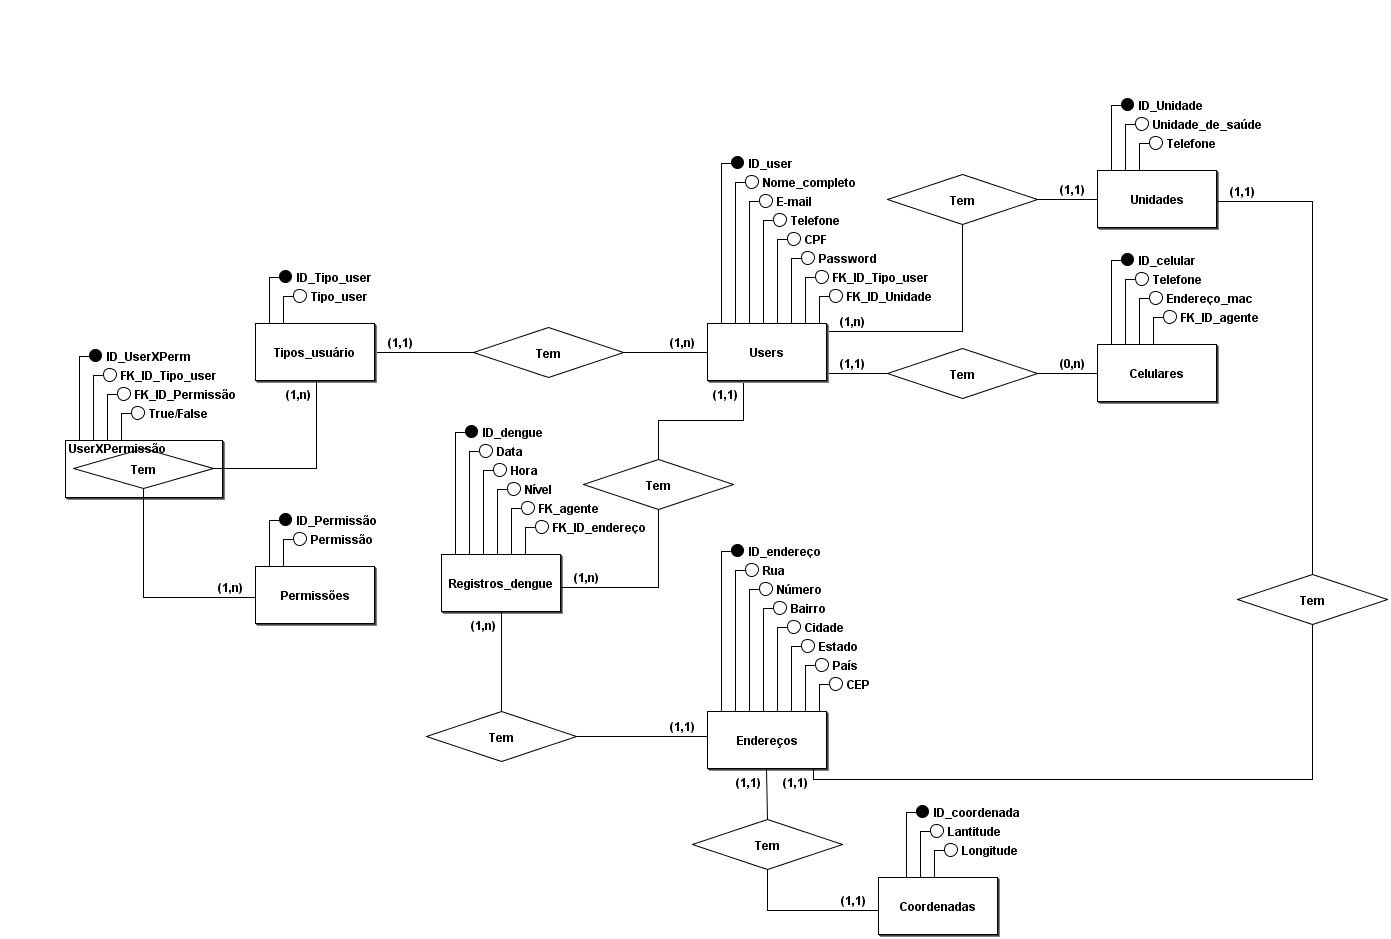
\includegraphics[width=1.0\linewidth]{Illustrations/Modelo_Conceitual Epidemix.png}
    \caption*{\textbf{Fonte: do próprio autor, 2024.}}
\end{figure}

\begin{figure}[H]
    \centering
    \caption{Banco de dados modelo lógico}
    \includegraphics[width=1.0\linewidth]{Illustrations/Modelo_Lógico_Epidemix.png}
    \caption*{\textbf{Fonte: do próprio autor, 2024.}}
\end{figure}

\vspace{12pt}

\textbf{Modelo de negócio Lean Canvas}\newline

O modelo de negócios Lean Canvas proporciona a clara compreensão de cada aspecto do modelo de negócio e dos elementos-chave do sistema EPIDEMIX. O objetivo é fornecer suporte de mapeamento com classificação de áreas de foco de dengue aos agentes de saúde de forma prática e simples, tanto no momento da administração dos dados quanto no momento de visualizá-los, por meio de dados em tempo real. Pretende-se utilizar o auxílio de inteligência artificial para gerar rotas entre os locais com focos da doença de forma eficiente, amenizando tempo e recursos. Ademais, buscamos fornecer outras informações importantes ao cliente por meio do WhatsApp, telefone ou reuniões. Canais de comunicação como mídias sociais e website foram estabelecidos. A atividade principal se baseia em um agente de saúde fazer o registro de uma localização com foco do Aedes aegypti em um mapa disponível na aplicação. Para isso, um dos recursos necessários é um dispositivo como celular, tablet ou computador com acesso à internet e GPS. O principal parceiro do sistema será o departamento de saúde pública. As despesas envolvem custos fixos, como salário de funcionários, hospedagem de website e hospedagem em servidor, internet (local e dados móveis), energia e locação de espaço, e também custos variáveis, como aquisição de hardwares e impostos. Em contrapartida, as fontes de renda variam entre o aluguel do software, aluguel de dispositivos para o registro dos dados e uma equipe para coleta e registro de dados, junto a um administrador/coordenador de equipes.

\begin{figure}[H]
    \centering
    \caption{Modelo de negócio Lean Canvas}
    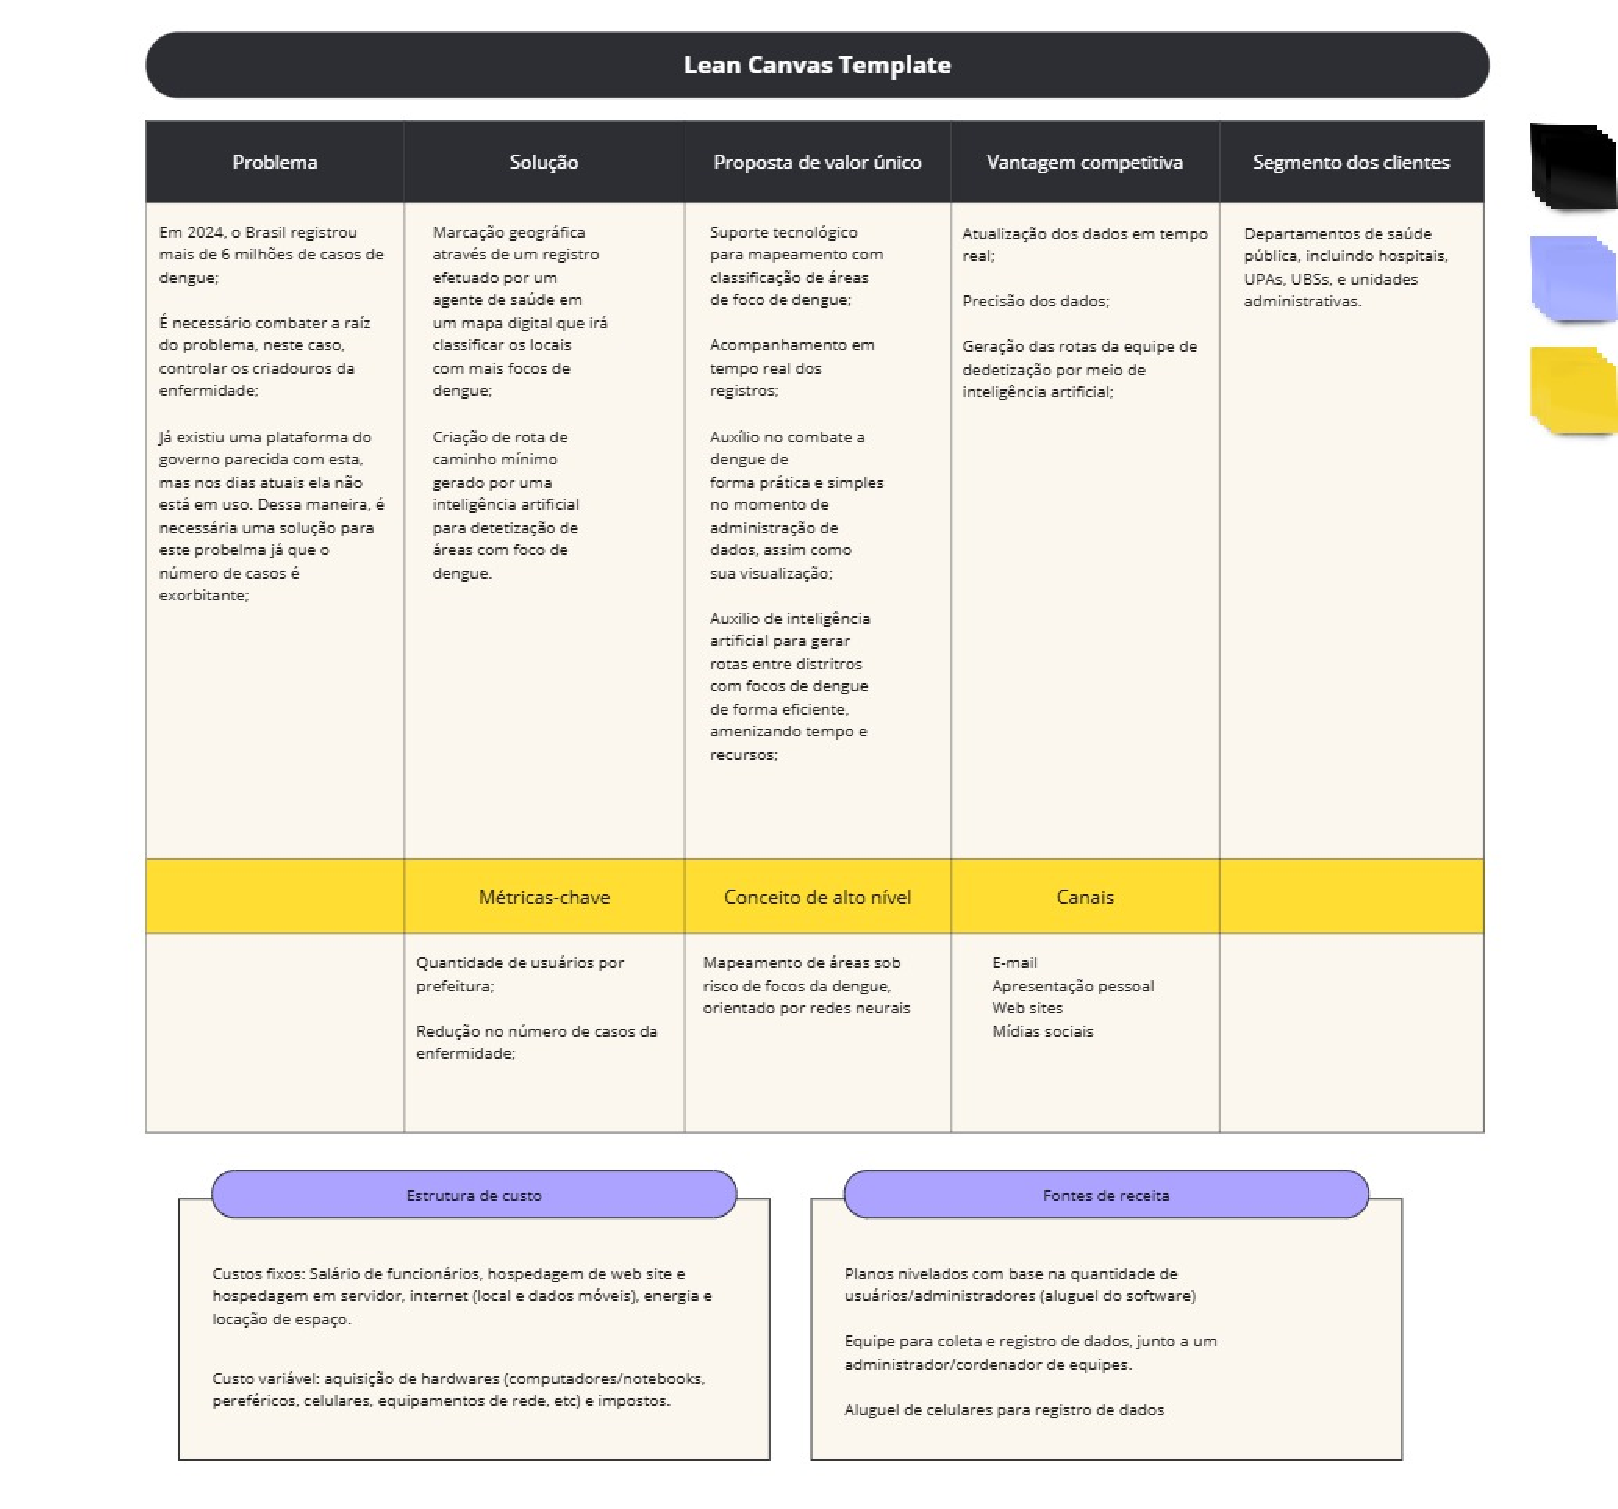
\includegraphics[width=1.0\linewidth]{Illustrations/Lean Canvas_Epidemix.pdf}
    \caption*{\textbf{Fonte: do próprio autor, 2024.}}
\end{figure}

\vspace{12pt}


 \section*{CONCLUSÃO}\label{sect:conclusao}

 Para auxiliar o cumprimento dos Objetivos de Desenvolvimento Sustentável (ODS) estabelecidos pela Organização das Nações Unidas (ONU), o trabalho busca favorecer a terceira meta, relacionada à saúde e bem-estar, por meio do mapeamento de áreas de foco de dengue e que contenham pessoas infectadas pela covid-19. 

O sistema será desenvolvido para que agentes de saúde possam registrar localizações no mapa que são afetadas pelas doenças, a fim de que, por meio do HeatMap, o administrador tenha acesso em tempo real às áreas de risco e organize os processos de dedetização de acordo com o nível de impacto em cada região. Sendo assim, com este sistema, pretende-se reduzir o número de óbitos pela doença transmitida pelo Aedes aegypti e pelo coronavírus no Brasil, além de facilitar o trabalho da equipe de saúde. O sistema busca ser o mais fácil possível para os usuários, onde o agente apenas aponta o local afetado, o gestor, por sua vez, simplesmente administra os dados, e o dedetizador visualiza as rotas para fazer o tratamento dos locais.  

 Toda a atividade é feita através da aplicação para dispositivos móveis, conhecida como EPIDEMIX, inclusive a visualização do mapa de calor pelo agente de dedetização. Entretanto, também existe a versão desktop destinada aos supervisores. Vale ressaltar que o aplicativo também estará disponível para usuários comuns, ou seja, aqueles que não são agentes de saúde, para que possam visualizar o mapa com as localizações de risco caso tenham interesse em preservar a saúde e evitar a contaminação por estas doenças.

Ao analisar o Modelo de Negócios Canvas, observa-se que o projeto ainda demanda testes práticos em contextos reais com agentes de saúde e seus respectivos gestores, para obter relatórios e avaliações, a fim de que a viabilidade operacional e econômica do sistema possa ser aprofundada.

Ademais, pensando na evolução contínua do sistema, observa-se a necessidade de realizar mais estudos sobre as doenças através de pesquisas de campo com os próprios agentes e gestores de saúde, reconhecendo especificidades ou técnicas que possam contribuir para a melhoria e precisão dos dados oferecidos pelo projeto, em especial reconhecer os níveis de intensidade da região afetada. Além disso, tais pesquisas fornecerão retorno sobre a eficácia e usabilidade do sistema na identificação de áreas de risco de dengue e covid-19 no Brasil.

Com o intuito de criar um sistema eficiente, pretende-se utilizar o conceito do caminho mínimo para determinar as rotas mais eficientes para as equipes de dedetização por meio de um grafo, onde os nós representam as áreas afetadas e as arestas as rotas viáveis. Dessa forma, será possível planejar rotas de maneira mais eficaz, permitindo que mais locais sejam tratados em menos tempo, facilitando o trabalho da equipe e contribuindo para o combate aos focos do Aedes e ao controle de casos de covid-19. No que se refere a identificar os dados de forma intuitiva em mapas de calor, propõe-se utilizar o processo de homogenização. Neste processo, as áreas não marcadas com uma localização receberão um valor estimado para criar uma representação contínua dos dados, suavizando as variações e permitindo uma melhor visualização das regiões afetadas. \cite{25}. \cite{26}

Espera-se que ao incluir as particularidades apresentados ao projeto, o sistema seja um fator significante na redução de número de óbitos por dengue e covid-19 no território brasileiro, e ainda, possa ser uma forma de facilitar o processo de reconhecimento de áreas afetadas por estas doenças de forma prioritária e em tempo real, a fim de contribuir para o controle de tais regiões, assim como garantir a eficácia do aplicativo.Cabe citar que se espera que as novas tecnologias incluídas futuramente possam ser reconhecidas como fatores cruciais que promoverão a eficácia e flexibilidade do aplicativo.

Em suma, conclui-se que testes práticos e pesquisas de campo para comprovar a viabilidade e usabilidade ainda são necessários. Entretanto, o estudo apresentado até o momento mostra-se uma alternativa com potencial contributivo ao oferecer suporte aos agentes de saúde e gestores na identificação de áreas de risco de dengue e covid-19, haja vista que o sistema busca facilitar a iniciativa do processo de dedetização dessas regiões.

\printbibliography

%% Elementos pós-textuais (opcionais): Apêndice e Anexo
%Caso for utilizar, basta retirar o símbolo de % na frente do comando
%%%%% Elementos pós-textuais
%%
%% Glossário, apêndices, anexos e índice remissivo (opcionais).

%% Apêndices
\begin{Appendix}

\section{Título de Apêndice}%
\label{sect:apx-a1}

Exemplo de apêndice (\Cref{sect:apx-a1}) em uma seção de \nameref{sect:appendix}.

\subsection{Título de Seção Secundária de Apêndice}%
\label{ssect:apx-a2}

Exemplo de seção secundária de apêndice (\Cref{ssect:apx-a2}).

\subsubsection{Título de Seção Terciária de Apêndice}%
\label{sssect:apx-a3}

Exemplo de seção terciária de apêndice (\Cref{sssect:apx-a3}).

\paragraph{Título de seção quaternária de Apêndice}%
\label{prgh:apx-a4}

Exemplo de seção quaternária de apêndice (\Cref{prgh:apx-a4}).

\subparagraph{Título de seção quinária de Apêndice}%
\label{sprgh:apx-a5}

Exemplo de seção quinária de apêndice (\Cref{sprgh:apx-a5}).

\end{Appendix}

%% Anexos
\begin{Annex}

\section{Título de Anexo}%
\label{sect:anx-a1}

Exemplo de anexo (\Cref{sect:anx-a1}) em uma seção de \nameref{sect:annex}.

\subsection{Título de Seção Secundária de Anexo}%
\label{ssect:anx-a2}

Exemplo de seção secundária de anexo (\Cref{ssect:anx-a2}).

\subsubsection{Título de Seção Terciária de Anexo}%
\label{sssect:anx-a3}

Exemplo de seção terciária de anexo (\Cref{sssect:anx-a3}).

\paragraph{Título de seção quaternária de Anexo}%
\label{prgh:anx-a4}

Exemplo de seção quaternária de anexo (\Cref{prgh:anx-a4}).

\subparagraph{Título de seção quinária de Anexo}%
\label{sprgh:anx-a5}

Exemplo de seção quinária de anexo (\Cref{sprgh:anx-a5}).

\end{Annex}

%% Índice remissivo
\printindex%


%% Fim do documento
\end{document}